\chapter{Experimental Setup}
\label{chap:Detector}
%\cite{Evans:2008zzb} \cite{LEP}
The hadron colliders aim at search for elementary particles and study the dynamics of interactions between them as predicted by the Standard Model or beyond the Standard Model theories. For the same beam energy, higher center-of-mass energy can be achieved in the hadron colliders as compared to the fixed target experiments. Due to the availability of very high center-of-mass energy of the colliding hadrons, it becomes possible for the researchers to understand the fundamental structure of the universe deeply and to look back in its history. The masses of the $Z$ and $W$ bosons, discovered by the UA1 and UA2 experiments \cite{Arnison:1983rp,Banner:1983jy}, were measured precisely at the Large Electron-Positron (LEP) collider. The experiment at proton-antiproton collider, Tevatron at FNAL discovered the top quark and also measured its mass. The search for the long awaited Higgs boson was carried out by the currently running most powerful accelerator, the Large Hadron Collider (LHC). Still many questions related to the the nature of dark matter, the existence of super-symmetry (SUSY) or the extra dimensions, are yet to be answered. 

The European Organization for Nuclear Research (CERN) is a world-class fundamental physics research organization founded in 1954. In the beginning, it concentrated on pure physics research to understand the inside of the atom, justifying the word ``nuclear'' in name. At present, the main area of research at CERN is particle physics which studies the fundamental constituents of matter and their forces of interactions. To accomplish this task, several particle detectors have been built by CERN which probe the physics at the TeV energy scale.

\section{The Large Hadron Collider}
The Large Hadron Collider (LHC) \cite{Evans:2008zzb} is the world's biggest and the most powerful particle accelerator and collider built by CERN. It occupies the circular tunnel between the border of France and Switzerland which was previously used by LEP collider \cite{LEP}. The circumference of the tunnel is 27 km and it lies underground at a depth ranging from 50 to 175 metres. The two beams of particles are accelerated in directions opposite to each other. There are 1,232 dipole to magnets maintain the beams in their circular path. The additional 392 quadrupole magnets are present to keep the beams focused to increase the probabilities of interaction between the particles. The LHC mainly collides proton beams, but it also collides proton-lead and lead-lead as well as xenon-xenon nuclei at different centre-of-mass energies. Since this thesis presents the study done using proton-proton (pp) collisions data, we will discuss the acceleration of protons only. 

The protons pass through a series of accelerators which increase their energy successively before their injection into the main ring of LHC. An overview of the various accelerators and detectors comprising the complex structure of the LHC is shown in Fig.~\ref{fig:LHC}. A bottle of hydrogen gas is the source of protons. The stripping of electrons from hydrogen gas atoms using an electric field yields protons. These protons are accelerated up to 100 keV through a radiofrequency quadrupole which provides the first focusing and a further acceleration to 750 keV energy. The linear particle accelerator (LINAC2) increases the energy of protons to 50 MeV. Then these protons are injected into the Proton Synchrotron Booster (PSB) in the form of bunches where they get accelerated to 1.4 GeV energy. The Proton Synchrotron (PS) further enhances the energy of protons to 25 GeV which is then increased to 450 GeV by the Super Proton Synchrotron (SPS). Finally the protons are injected into two beam pipelines of the main LHC ring where their energy increases to the beam energy. The total center-of-mass energy in head-on collisions between beams of same mass particles is twice the energy of the beams. 

\begin{figure}[!h]
 \begin{center} 
 \hspace*{-12mm}
 \vspace{4mm}
 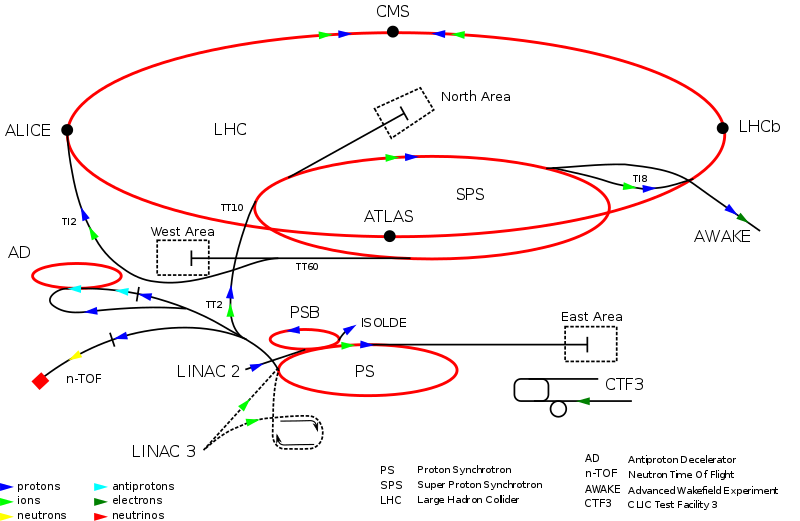
\includegraphics[width=1.2\textwidth]{/home/anter/Desktop/Thesis/Figures/LHC.png}\\
 \vspace*{5mm}
 \caption[An overview of the different experiments of the Large Hadron Collider (LHC), a complex particle accelerator and collider located at CERN.]{An overview of the different experiments of the Large Hadron Collider (LHC), a complex particle accelerator and collider located at CERN\footnotemark.}
 \label{fig:LHC}
 \end{center}
\end{figure}
\footnotetext{Source : \url{https://en.wikipedia.org/wiki/Large_Hadron_Collider}}

The accelerated beams collide at four interaction points around which six detectors are located : ALICE (A Large Ion Collider Experiment) \cite{Aamodt:2008zz}, ATLAS (A Toroidal LHC Apparatus) \cite{Aad:2008zzm}, CMS (Compact Muon Solenoid) \cite{Chatrchyan:2008aa,Bayatian:2006nff,Ball:2007zza}, LHCb (Large Hadron Collider for Beauty) \cite{Alves:2008zz}, LHCf (Large Hadron Collider forward)\cite{Adriani:2008zz} and TOTEM (Total, elastic and diffractive cross-section measurement) \cite{Anelli:2008zza}. The CMS and ATLAS are two general purpose detectors dedicated to the validation of the Standard Model theory predictions, existence of super-symmetry (SUSY) and also looking for extra dimensions. The ALICE is a heavy-ion detector which studies quark-gluon plasma, a state of matter believed to be present just after the Big Bang, produced in collisions of lead ions. The LHCb experiment will explore the differences between matter and antimatter and new physics through b-quark (beauty) studies. TOTEM experiment is dedicated to cross-section measurements whereas LHCf focuses on forward physics. 

The LHC successfully injected the first protons on September 10, 2008 but after few days there was magnetic quench in bending magnets which lead to a loss of $\sim$6 tonnes of liquid helium. After recovery from this incident, at first the low-energy beams were circulated in the tunnel on November 20, 2009 and after three days the first collisions took place in all four detectors at \cme = 450 GeV. The LHC achieved 1.18 TeV energy per beam on November 30, 2009. This made LHC the world’s highest energy particle accelerator and left behind the Tevatron having record of 0.98 TeV per beam for eight years. The LHC recorded pp collisions at \cme = 2.36 TeV around December 15, 2009. After this the beam energy was ramped up to 3.5 TeV on March 19, 2010 which resulted in the first pp collisions at \cme = 7 TeV on March 30, 2010. The beam energy was kept at 3.5 TeV throughout 2011, and increased to 4 TeV in 2012. After a long shutdown for two years, the LHC restarted in 2015 and collided the proton beams at a much higher center-of-mass energy of 13 TeV and is running successfully till now. In the coming years, protons will be made to collide at a designed \cme = 14 TeV with luminosity up to 10$^{34}$ cm$^{-2}$s$^{-1}$. In this thesis, work has been carried out using the pp collisions data collected by the CMS detector at \cme = 8 TeV in the year of 2012.

\subsection{Luminosity Measurement}
\label{sec:lumi}
Luminosity (\lumi) is one of the most important parameters of an accelerator which characterizes its performance. It defines the rate at which collisions occur and is given by the number of collisions produced in a detector per cm$^2$ and per second. Cross-section ($\sigma$) is a measure of the probability that an event can take place. \lumi is related to total number of events $N$ of a process over a time period T and $\sigma$ as :
\begin{equation}
N = \int_{0}^{T} \lumi~\sigma~dt = \lumi_{int}~\sigma
\end{equation}
where $\int_{0}^{T} \lumi~dt = \lumi_{int}$ gives the total integrated luminosity. \lumi$_{int}$ is expressed in the units of area, usually in barn$^{-1}$ and gives a direct indication of number of events produced in a process. For example, an integrated luminosity of 10 fb$^{-1}$ means that 10 events are produced in a process having cross-section equal to 1 fb.

The luminosity depends on the particle beam parameters as :

\begin{equation}
\lumi = \frac{N_b~N^2_p~f_{rev}~\gamma~F}{4\pi~\epsilon_n~\beta^*}
\end{equation}
where $N_b$ is the number of bunches per beam, $N_p$ is the number of particles in each bunch, $f_{rev}$ is the revolution frequency of the beam, $\gamma$ is the relativistic gamma factor and $F$ is the geometric luminosity reduction factor. The effective collision area of the two beams is related to the normalized transverse beam emittance $\epsilon_n$ and the value of the betatron function $ \beta^*$ at the interaction point.
 
The CMS experiment constantly monitors the instantaneous luminosity delivered by LHC which is shown versus time in Fig.~\ref{fig:lumi} for proton-proton collisions at nominal center-of-mass energy for the years 2010-2017. The relative instantaneous luminosity is calculated by using two methods \cite{CMS:2013gfa} : Hadron Forward (HF) method by measuring the particle flux in the hadron forward calorimeter and Counting method where the number of reconstructed vertices in the pixel tracker are counted. The measurement of the absolute luminosity is performed using van-der-Meer scans done in special runs of the LHC \cite{vanderMeer:1968zz}. The uncertainty on the measured luminosity for 2012 data set is 2.5\% (syst.) and 0.5\% (stat.).

\begin{figure}[!h]
 \begin{center}
 \vspace*{4mm} 
 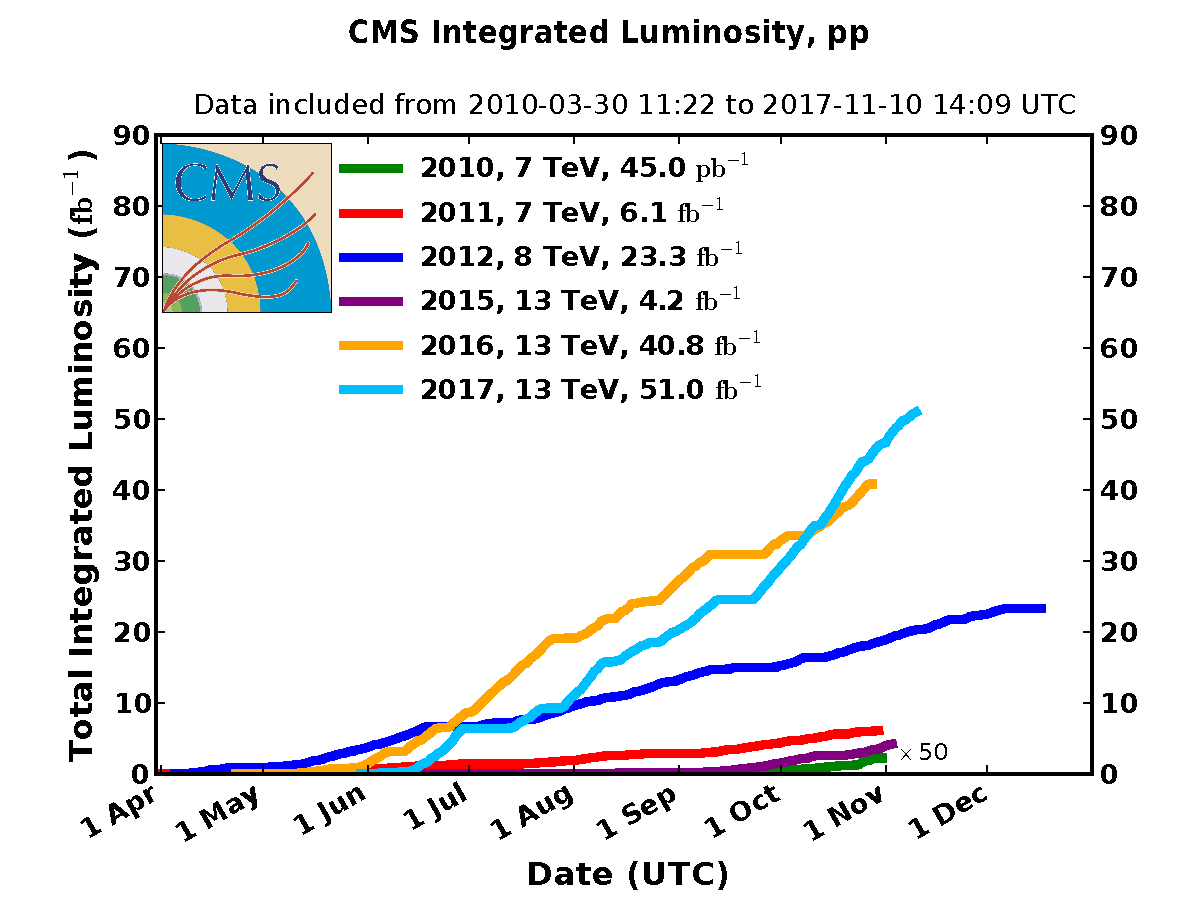
\includegraphics[width=.8\textwidth]{/home/anter/Desktop/Thesis/Figures/int_lumi_cumulative_pp_2.pdf}\\
 \vspace*{5mm}
 \caption[The integrated luminosity delivered by stable beams to CMS during proton-proton collisions.]{The integrated luminosity delivered by stable beams to CMS during proton-proton collisions taking place at nominal center-of-mass energy, is shown versus time for data-taking in 2010 (green), 2011 (red), 2012 (blue), 2015 (purple), 2016 (orange) and 2017 (light blue) run periods of the LHC\footnotemark.}
 \label{fig:lumi}
 \end{center}
\end{figure}
\footnotetext{Source : \url{https://twiki.cern.ch/twiki/bin/view/CMSPublic/LumiPublicResults}}
\subsection{Pileup Interactions}
\begin{figure}[!h]
 \begin{center}
 \vspace*{0mm} 
 %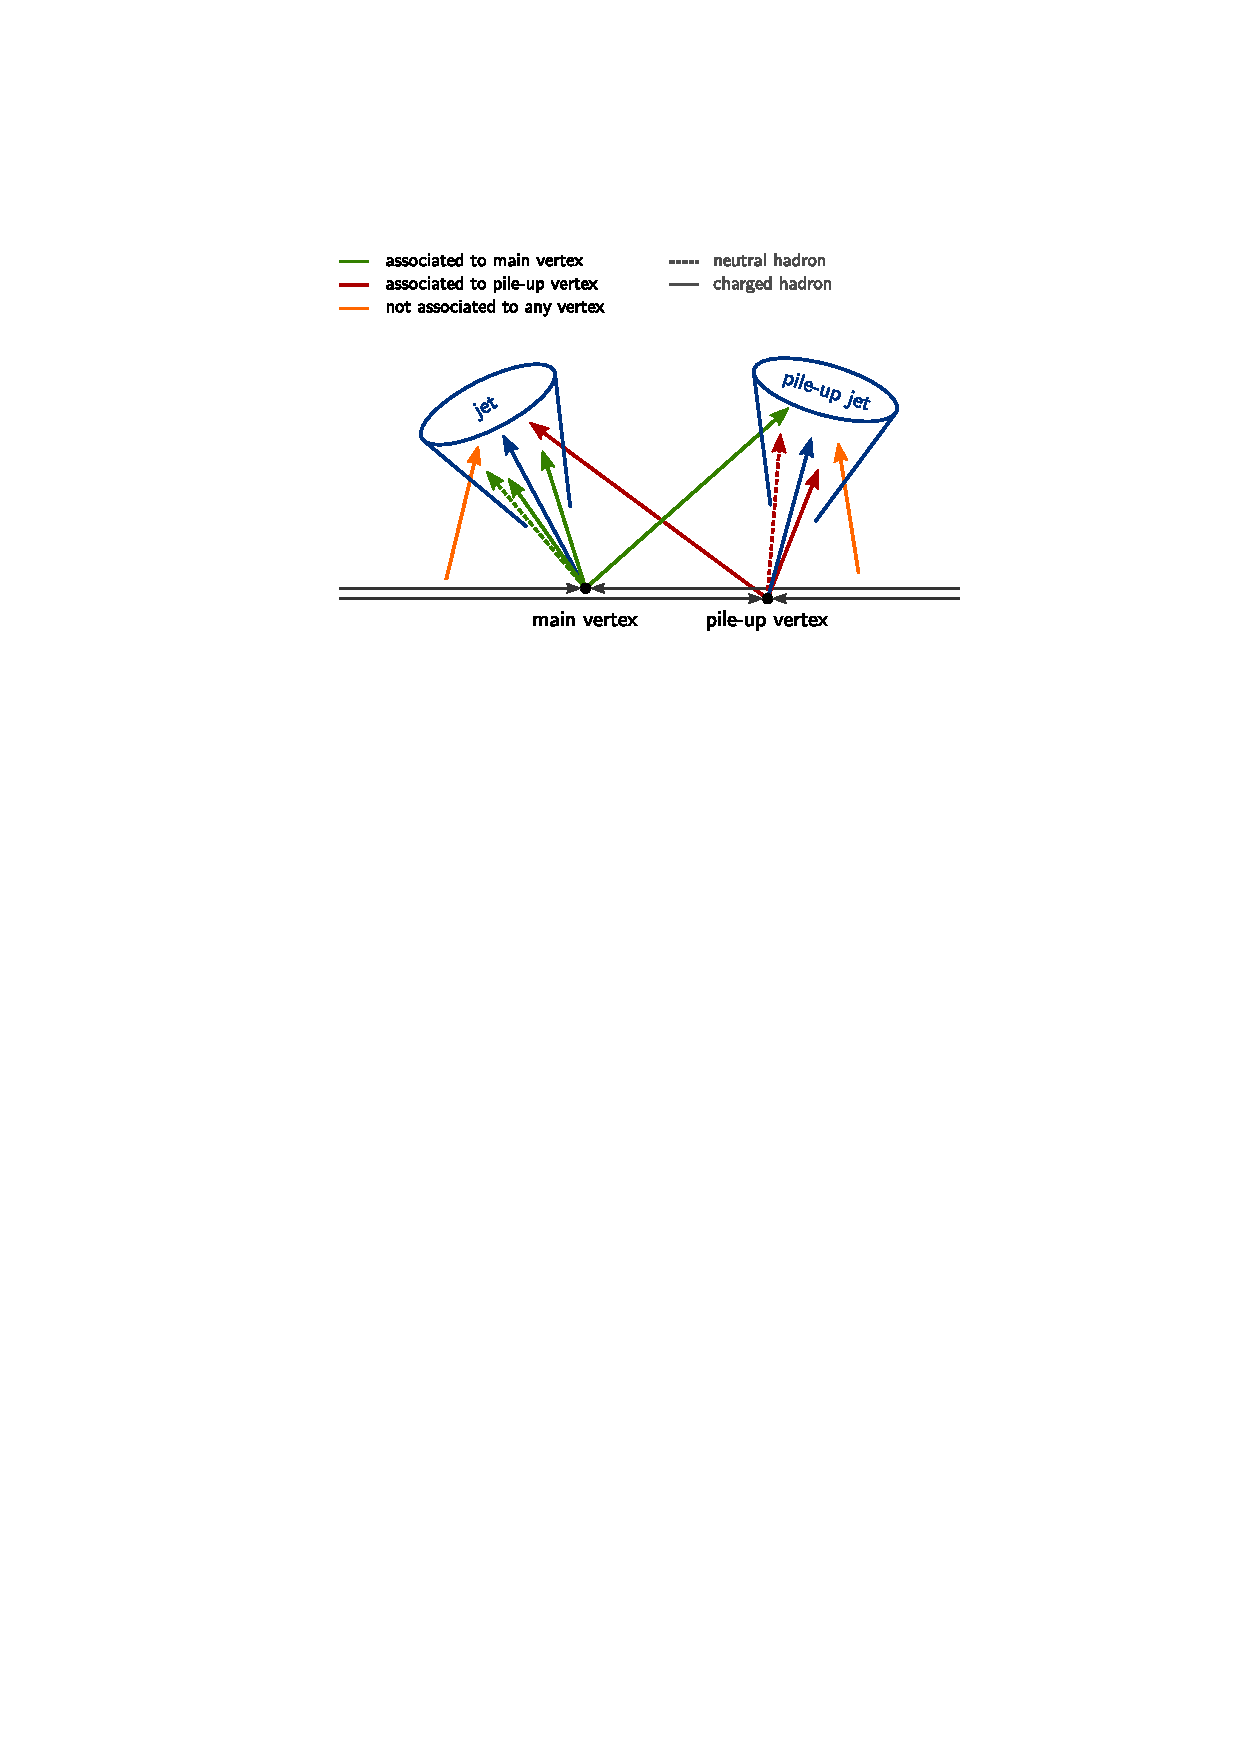
\includegraphics[width=.8\textwidth]{/home/anter/Desktop/Thesis/Figures/cropped_Pileup.pdf}\\
 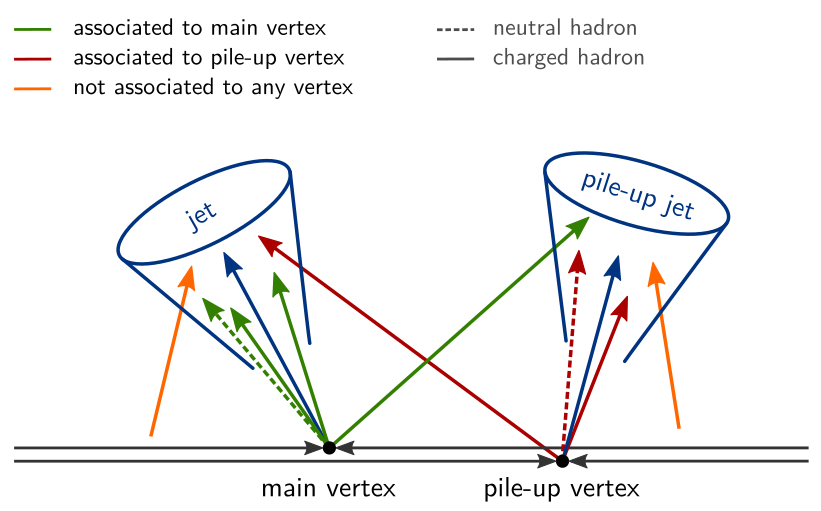
\includegraphics[width=.8\textwidth]{/home/anter/Desktop/Thesis/Figures/Final/Pileup.png}\\
 \vspace*{5mm}
 \caption[In a proton-proton collision, the particles produced from the hard interaction are clustered into a jet. The hard interaction corresponds to the main vertex. The particles produced in the interactions other than the hard one, form a pileup jet.]{In a proton-proton collision, the particles produced from the hard interaction are clustered into a jet. The hard interaction corresponds to the main vertex. The particles produced in the interactions other than the hard one, form a pileup jet\footnotemark.}
 \label{fig:pileup_d}
 \end{center}
\end{figure}

To observe the extremely rare events, the event rate in a collider should be very high. This demands delivered luminosity to be high which is achieved by increasing the number of bunches or increasing the number of protons per bunch. However, this comes at the cost of multiple proton-proton interactions coming from independent hadron-hadron collisions occurring in the same bunch crossing, called pileup (PU) interactions. The hard interaction in every event is accompanied by a large amount of PU interactions which give rise to low \pt jets. The vertex of pileup interaction is reconstructed from tracks pointing to it as shown in Fig.~\ref{fig:pileup_d}. The pileup due to the additional collisions within a single bunch crossing is called in-time pileup whereas pileup coming from collisions other than hard scattering in other bunch crossings is known as out-of-time pileup. The pileup itself cannot be directly measured, it can be correlated to various other directly measurable quantities. The number of primary vertices ($N_{PV}$) is directly related to the amount of pileup as the pileup comes from the additional proton-proton interactions. The greater the $N_{PV}$, the more pileup energy is added to the jets which needs to be subtracted. 
\footnotetext{Source : \url{http://cds.cern.ch/record/1747055}}

\section{The Compact Muon Solenoid}
The Compact Muon Solenoid (CMS) detector is a general purpose detector located at the interaction point 5 (P5) of the main LHC ring, near the village of Cessy in France. The name of CMS comes from its compact size with main emphasis on the detection of muons and enclosed within high solenoidal magnetic field. The CMS detector aims at identifying the different types of particles produced in proton-proton and heavy ion collisions and measuring their energies and momenta. This is achieved by concentric layers of different sub-detectors arranged in a cylindrical complex structure with 21.6 m length and 15 m diameter. The silicon-based tracker surrounds the the interaction point and forms the innermost layer. After the tracker, there are layers of a scintillating crystal electromagnetic calorimeter (ECAL) and a sampling hadron calorimeter (HCAL). The calorimeters are enclosed inside the superconducting solenoid. Outside the magnet lies the large muon detectors embedded inside an iron yoke. 
\begin{figure}[!h]
\begin{center}
\vspace{1mm}
\hspace*{-6mm}
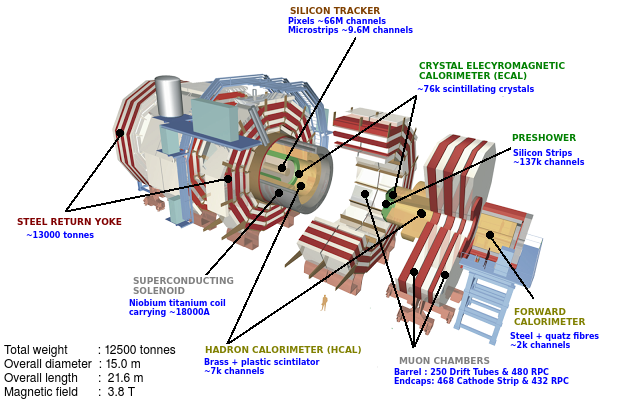
\includegraphics[scale = 0.98]{/home/anter/Desktop/Thesis/Figures/CMS_2_new.png}\\
\vspace*{5mm}
\caption[The three dimensional view of the CMS detector along with its sub-detector components.]{The three dimensional view of the CMS detector along with its sub-detector components\footnotemark.}
\vspace{-3mm}
\label{fig:CMS}
\end{center}
\end{figure}The three dimensional view of the CMS detector along with its components is presented in Fig.~\ref{fig:CMS}. The CMS was constructed in parts at ground and assembled later on in the cavern. The components are easily accessible for upgrades or repairs as the detector can be opened up into movable slices. Figure~\ref{fig:CMS_front} shows the front view of the CMS detector differentiating individual components which contribute to event reconstruction. The dashed and solid lines represent the invisible and visible tracks, respectively, of the reconstructed particles. The different particles are : photons ($\gamma$), muons ($\mu^{\pm}$), electrons (e$^{-}$), neutrons (n) and charged hadrons (pions $\pi^{\pm}$).

\begin{figure}[!h]
\begin{center} 
\hspace*{-15mm}
\vspace{4mm}
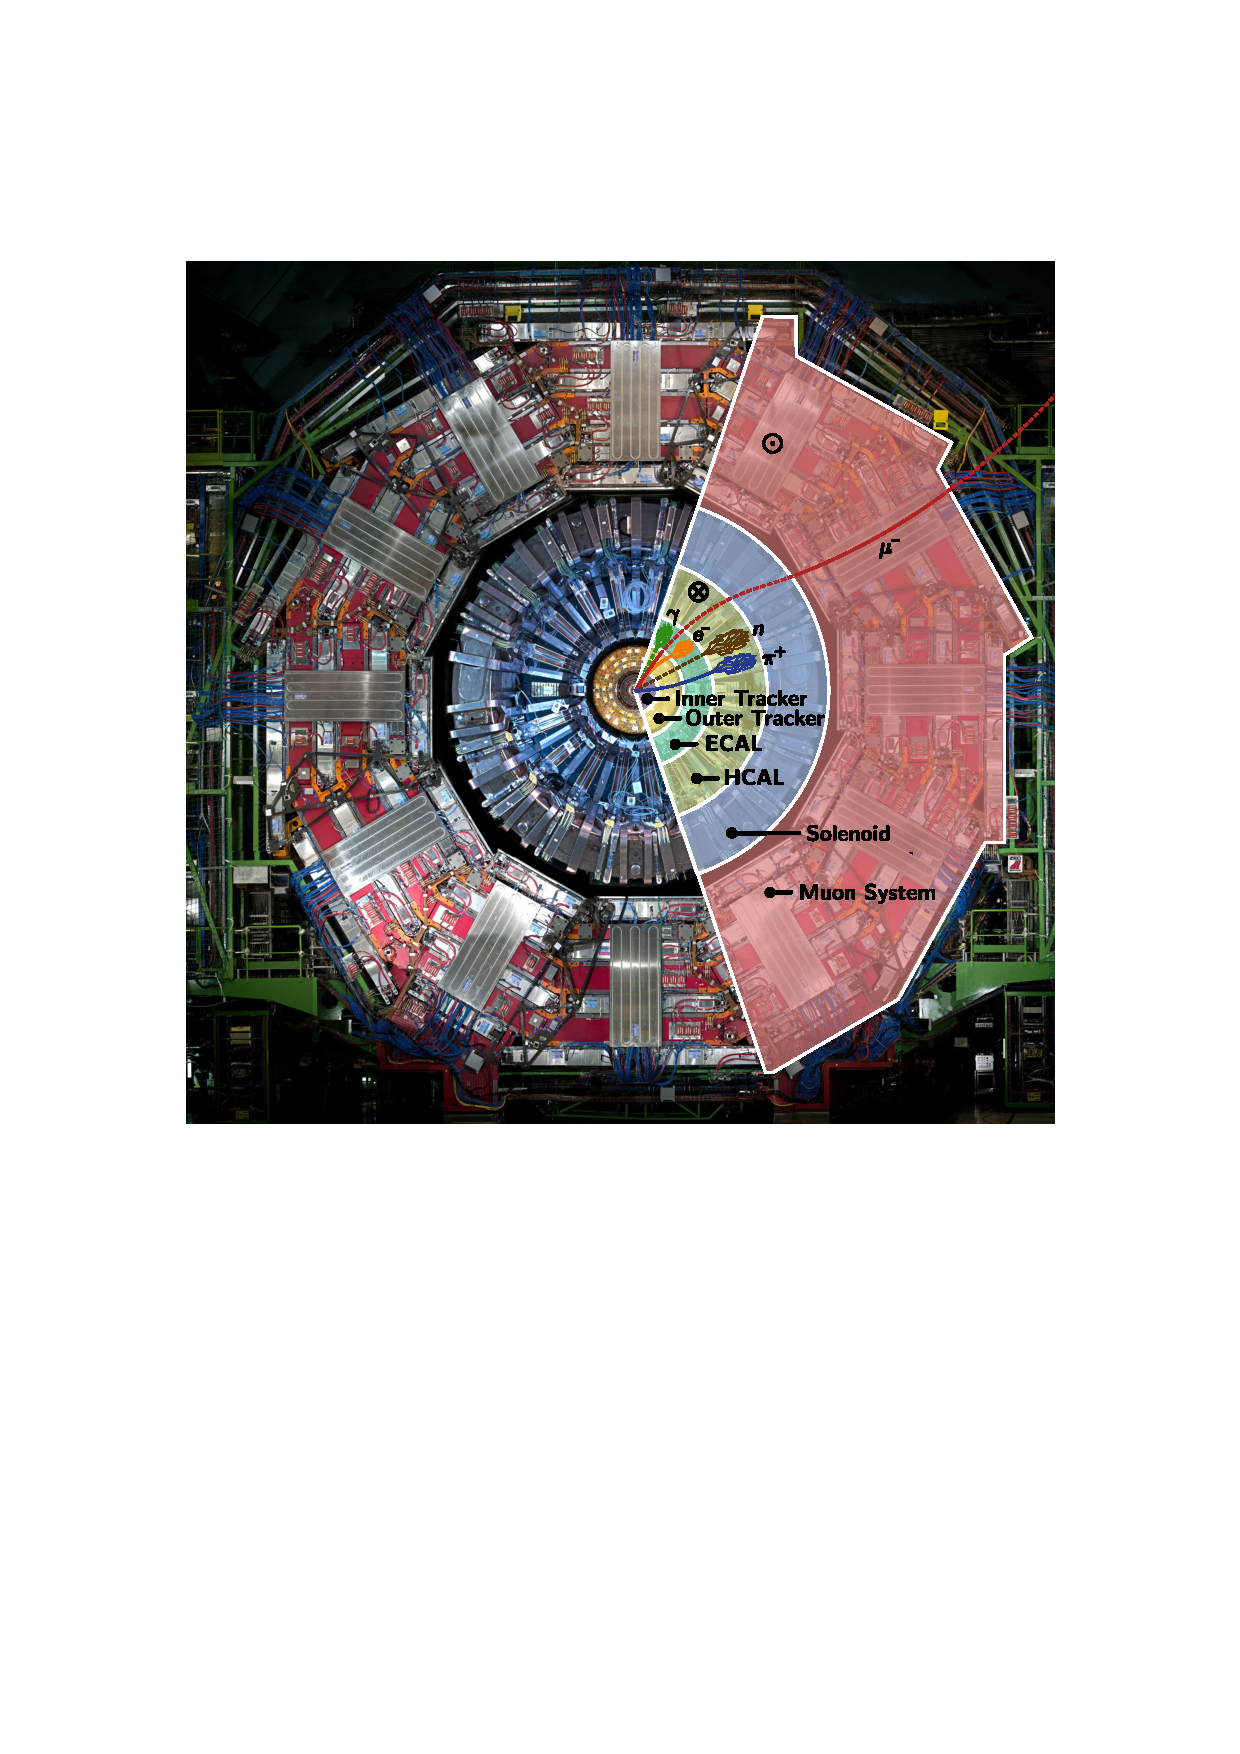
\includegraphics[scale = 0.55]{/home/anter/Desktop/Thesis/Figures/cropped_CMS_Front.pdf}
\vspace{3mm}
\caption[Front view of the CMS detector along with its various components.]{Front view of the CMS detector along with its components : inner tracker, outer tracker, electromagnetic calorimeter, hadronic calorimeter, solenoid and muon system. The path of different particles detected by dedicated sub-detectors are shown by dashed (invisible track) and solid (visible track) lines. $\otimes$ and $\odot$ gives the direction of magnetic field inside the solenoid and in the return yoke, respectively. Taken from \cite{Ball:2007zza}.}
\label{fig:CMS_front}
\end{center}
\end{figure}
A brief overview of the CMS detector has been presented and the details of the its design as well as physics performance are available in Ref.~\cite{Bayatian:2006nff,Ball:2007zza}. Before going into the details of each sub-detector, first the CMS coordinate system is described in the next section.
\vspace{1mm}
\subsection{Coordinate System}
\footnotetext{Source : \url{https://orbiterchspacenews.blogspot.in/2013/04/cern-cms-prepares-for-future.html}}
A right-handed coordinate system, illustrated in Fig.~\ref{fig:coordinate}, is used by the CMS detector. The origin of the co-ordinate system lies at the nominal interaction point (IP) of the collisions. The $x$-axis points horizontally from the I and towards the center of the LHC ring. The $y$-axis points vertically upwards and the $z$-axis along the beam direction towards the Jura mountains. %The radial coordinate in $x$-$y$ plane is denoted by $r$. 
Following customary polar coordinate conventions : the azimuthal angle $\phi$ is measured from the $x$-axis in the $x$-$y$ plane as $\phi = {\rm tan^{-1}}(\frac{y}{x})$ where $\phi$ = 0 points to the \plusn $x$ axis and $\phi$ = $\pi$/2 points to the \plusn $y$ axis. The polar angle $\theta$, is calculated from the $z$-axis in the $z$-$y$ plane as $\theta~=~{\rm tan^{-1}}\big(\frac{x^2~\plus y^2}{2}\big)$ with $\theta$ = 0 corresponding to the \plusn $z$ direction and $\theta$ = $\pi$ to the -$z$ direction. The quantities rapidity $y$ and the pseudorapidity $\eta$ are preferred over the angles $\theta$ and $\phi$. The rapidity and pseudorapidity are given by Eq.~\ref{eq:pseudorap}. Both the quantities are equal for massless particles.
\begin{equation}
\begin{gathered}
y = \frac{1}{2}~{\rm ln} \bigg(\frac{E~\plus p_z}{E - p_z} \bigg) \\
\eta = -~{\rm ln}\bigg({\rm tan}\bigg(\frac{\theta}{2}\bigg)\bigg)
\end{gathered}
\label{eq:pseudorap}
\end{equation}
\begin{figure}[!h]
\begin{center} 
\hspace*{-15mm}
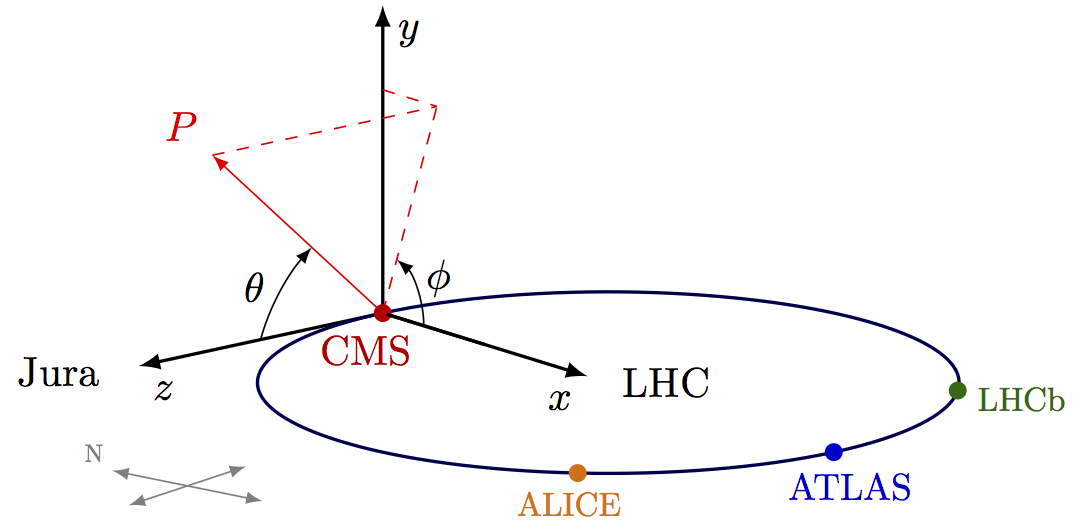
\includegraphics[scale = 1.5]{/home/anter/Desktop/Thesis/Figures/cms_coordinate_system.png}
\vspace{3mm}
\caption[The right-handed coordinate system used by the CMS detector.]{The CMS detector uses the right-handed coordinate system\footnotemark having origin at the interaction point (IP). The $x$-axis points horizontally from the IP towards the center of the LHC ring, the $y$-axis points vertically upwards whereas the $z$-axis along the beam direction towards the Jura mountains. The azimuthal angle $\phi$ is measured from the $x$-axis in the $x$-$y$ plane and the polar angle $\theta$ is calculated from the $z$-axis in the $z$-$y$ plane.}
\label{fig:coordinate}
\end{center}
\end{figure}
The difference between rapidities $\Delta y$ is invariant under longitudinal Lorentz boost whereas it does not hold for $\eta$. Hence $y$ is considered in this thesis. The angular distance between the two particles is defined by $\Delta R = \sqrt{(\Delta \eta)^2~\plus (\Delta \phi)^2}$. The momentum component transverse to the direction of beam \pt, is computed from the $x$- and $y$-components as \pt = $\sqrt{p^2_x~\plus p^2_y}$ and the transverse energy is given by $E_T$ = $E$ sin$\theta$. After introducing the CMS coordinate system, further the detector subsystems are described briefly in the following sections. In Fig.~\ref{fig:CMS_quad}, a longitudinal section of the CMS detector shows the location of different sub-systems along with the superconducting solenoid, in the $y$-$z$ plane. 
\footnotetext{Source : \url{https://wiki.physik.uzh.ch/cms/latex:example_spherical_coordinates}}
\begin{figure}[!h]
\vspace*{3mm}
\begin{center} 
\hspace*{-5mm}
%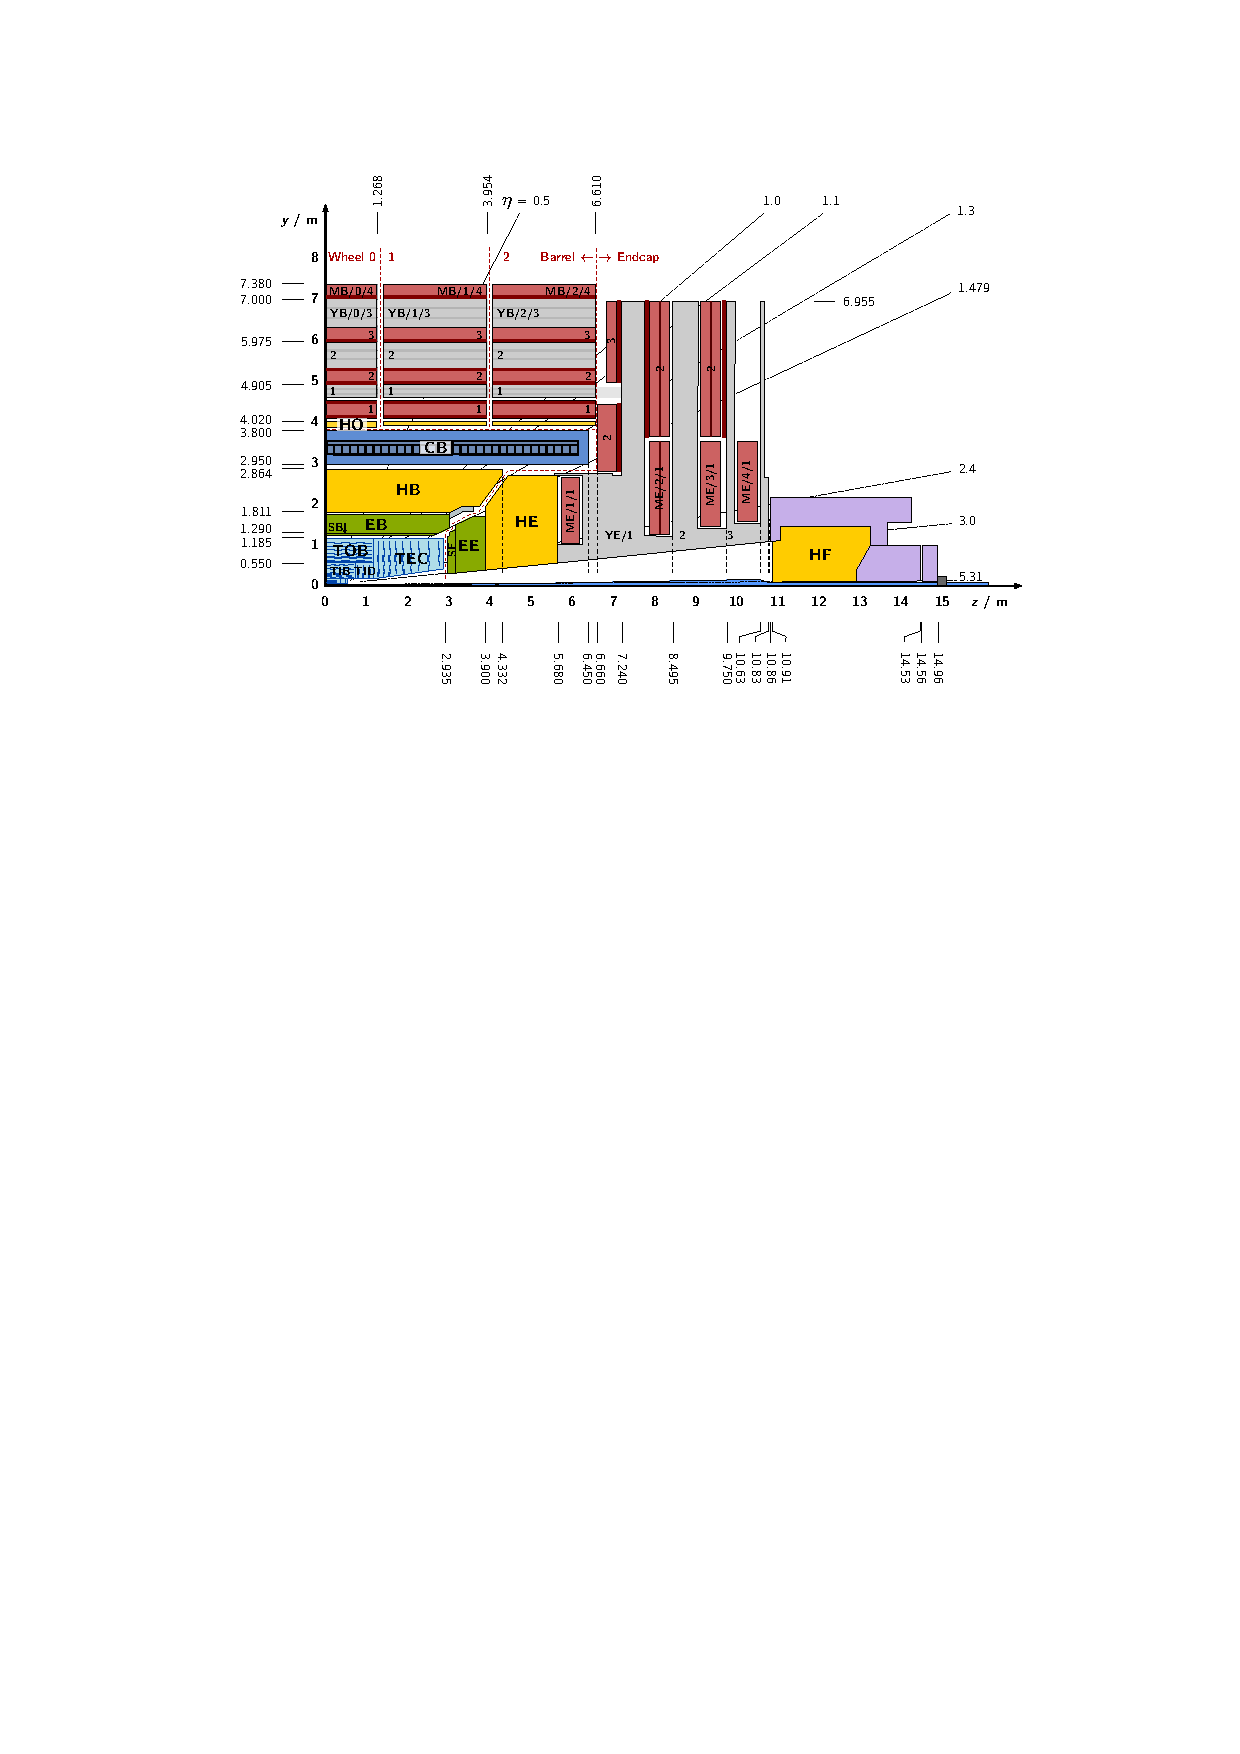
\includegraphics[scale = 1.1]{/home/anter/Desktop/Thesis/Figures/cropped_CMS_Quad.pdf}\\
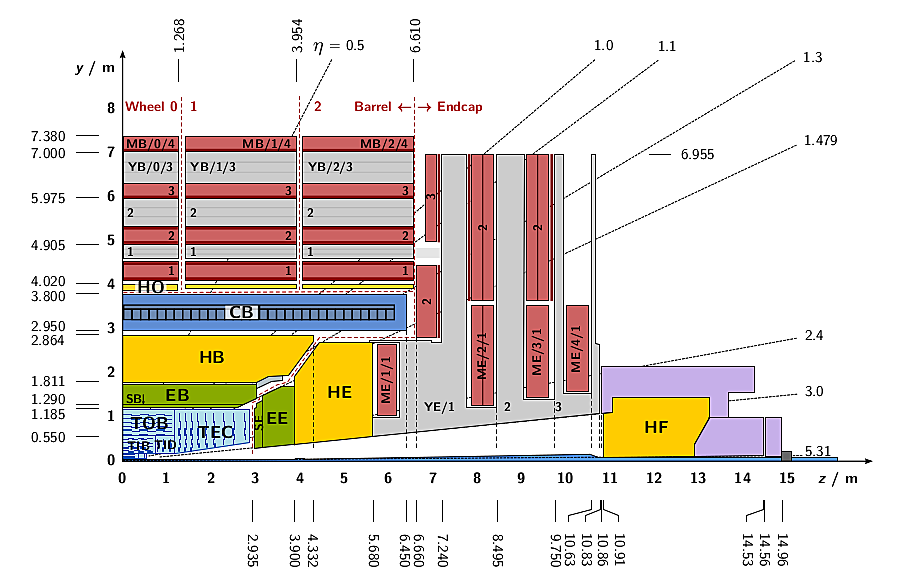
\includegraphics[scale = 0.62]{/home/anter/Desktop/Thesis/Figures/Final/CMS_Quad.png}
\vspace*{5mm}
\caption[A longitudinal view of the CMS detector is shown in the $y$-$z$ plane.]{A longitudinal view of the CMS detector is shown in the $y$-$z$ plane\footnotemark. It shows the tracking detector (TIB, TID, TOB, TEC) close to the nominal interaction point at (0,0), the electromagnetic (EB, EE) and hadronic (HB, HE, HO, HF) calorimeters. The coil of the solenoid magnet (CB) surrounds the inner barrel region. The iron return yoke (YB, YE) is interleaved with the muon chambers (MB, ME).}
\label{fig:CMS_quad}
\end{center}
\end{figure}

\subsection{Inner Tracker System}
The charged particles produced from the LHC collisions leave their trajectories as they move outward from the interaction point. The particle flux within the detector decreases as 1/$r^2$. So the tracks of the particles need to be measured as close to the collision point as possible and in a precise manner. The innermost tracking system of the CMS consists of silicon detectors and measures the hits produced by the charged particles. It surrounds the interaction point and has a cylindrical volume of length of 5.8 m and a diameter of 2.5 m and covers a pseudorapidity range up to $|\eta|$ \ls 2.5. The passage of the charged particles through the silicon detector material produces small ionization currents which get detected as hits. Such multiple hits when combined, reconstruct the track which gives the information about the direction and transverse momentum \pt of the charged particle. Silicon detectors have a much higher resolution in tracking charged particles as compared to the older ones such as cloud chambers or wire chambers.\footnotetext{Source : \url{http://cds.cern.ch/record/1747055}} CMS inner tracking system shown in Fig.~\ref{fig:tracker} consists of two sub-systems :\\ \newline 
{\bf Pixel Detector -} A pixel detector is located close to the beam pipe. It has three co-centric barrel layers lying at radii of 4.4, 7.3 and 10.2 cm from the beam pipe. \begin{figure}[h]
\begin{center} 
\vspace*{2mm}
\hspace*{-6mm}
%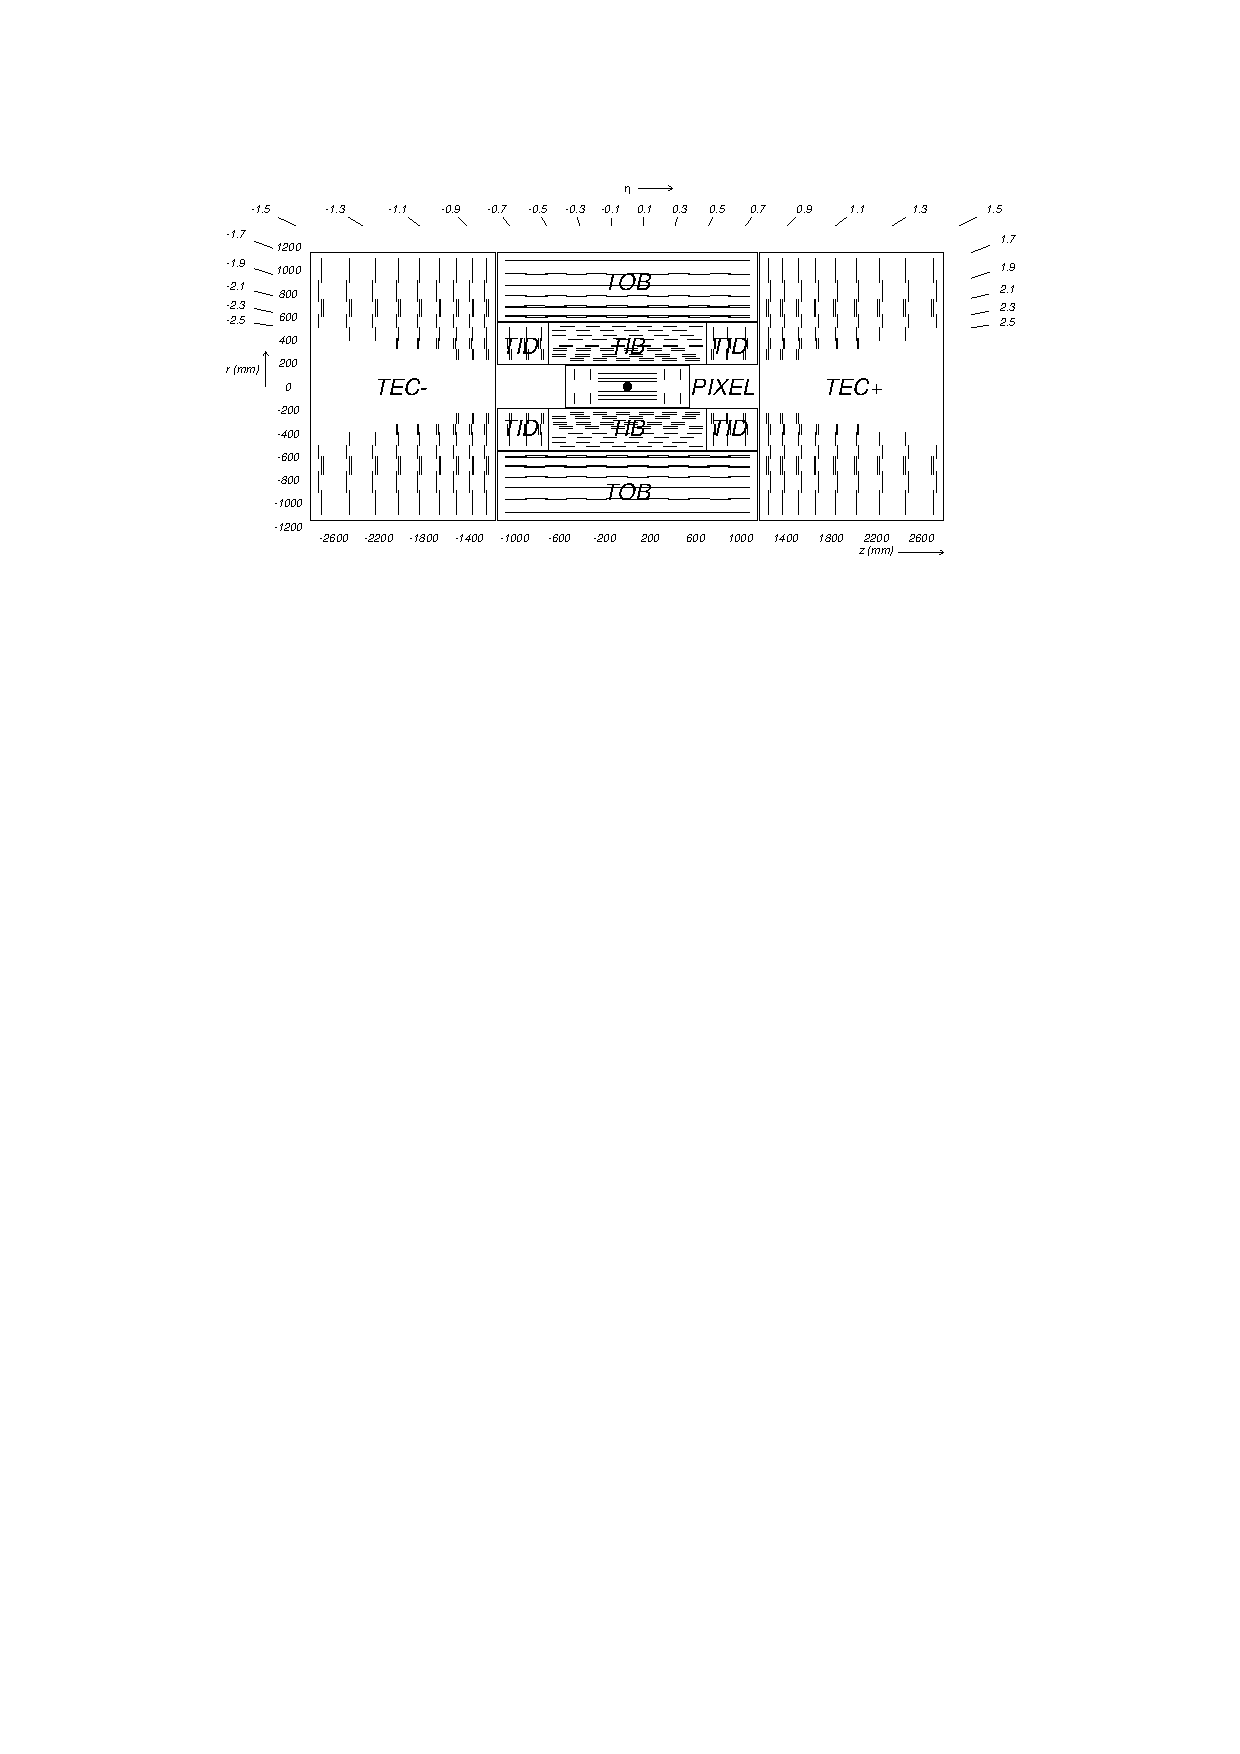
\includegraphics[scale = 1.1]{/home/anter/Desktop/Thesis/Figures/cropped_Tracker.pdf}\\
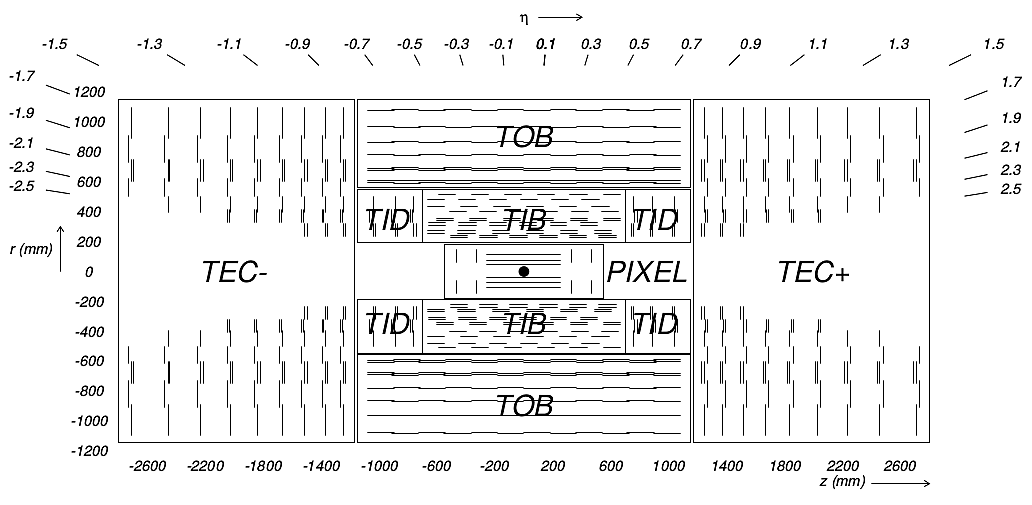
\includegraphics[scale = 0.55]{/home/anter/Desktop/Thesis/Figures/Final/Tracker.png}
\caption[A longitudinal view of the inner tracking system is shown in $r$-$z$ plane.]{A longitudinal view of the inner tracking system is shown in $r$-$z$ plane. The CMS tracking system is made up of the silicon pixel detector and the silicon strip detector  The silicon strip detector has four components : The Tracker Inner Barrel (TIB) complemented by the Tracker Inner Disks (TID) which are further surrounded by the Tracker Outer Barrel (TOB) in barrel region. Tracker End Cap (TEC) covers high $\eta$ ranges up to $\eta$ = 2.5. Taken from \cite{Chatrchyan:2008aa}.}
\label{fig:tracker}
\end{center}
\end{figure} It has two disks of pixel modules on each side of barrel. Taking the design luminosity of LHC i.e. 10$^{34}$ cm$^{-2}$s$^{-1}$, about 1000 particles are produced from more than 20 overlapping proton-proton collisions. These particles traverse through the tracker for each bunch crossing, i.e. every 25 ns. The size of each pixel is 100 $\micro$m (in $r$,$\phi$) $\times$ 150 $\micro$m (in $z$) which gives an average occupancy of 10$^{-4}$ per bunch crossing. Due to the large Lorentz effect, the pixel tracker has a spatial resolution of 10 $\micro$m and 20 $\micro$m in ($r$,$\phi$) and $z$ plane respectively, which is beneficial for a precise determination of the primary and secondary vertices and good momentum resolution. \\ \newline
{\bf Strip Detector -} After coming out of the pixel detector the charged particles traverse through ten layers of silicon strip detectors, reaching out to a radius of 130 cm. The silicon strip detector has four layers of inner barrel (TIB) assembled in shells with two inner endcaps (TID), each having three small discs. There is an outer barrel tracker (TOB) consisting of six concentric layers. Finally two endcaps (TEC) are placed at the end of tracker. Each part of the tracker has silicon modules which are designed with dedicated functions. The strip detector performs the measurement of the particle tracks with a reduced resolution of 23 $\micro$m which hints the smaller particle flux at larger distances from the collision point.
The active silicon area of CMS tracker is about 200m$^{2}$ which makes it the largest silicon tracker. Along with the measurement of tracks, the energy also needs to be measured for which the calorimeters are present outside the tracker. To measure the momenta of the particles precisely, they should interact with the tracker to a minimum extent. In contrast, to measure their energy, they are required to interact with the calorimeters fully.

\subsection{Electromagnetic Calorimeter}
The electromagnetic calorimeter (ECAL) is a homogeneous and hermetic calorimeter used to slow down the produced photons and electrons/positrons and measure their energy by absorbing them into the detector material. The barrel part of the ECAL is made up of 61200 lead tungstate (PbWO$_4$) crystals and each of the two end caps has 7324 crystals. PbWO$_4$ is a very dense material having a short radiation length of X$_0$ = 0.89 cm and covers the pseudorapidity up to $|\eta|$ \ls 3.0. The incorporation of oxygen makes it highly transparent and enables to emit scintillation light. The small Moli$\grave{e}$re radius of 2.19 cm of this material, gives a fine granularity. These properties leads to compact size of ECAL so that it can be easily placed within the solenoid magnet. 

When the electrons, positrons or photons produced in the collisons, hit the crystals of ECAL, they produce electromagnetic showers through the subsequent processes of bremsstrahlung and electron-positron pair production. The energy of the particles deposited by the photoelectric effect and the Compton scattering causes excitation of the material atomic state and the emission of photons. The number of emitted photons is directly proportional to the energy of the incident particles. The emitted photons are detected by silicon avalanche photo diodes (APDs) in the barrel region and vacuum phototriodes (VPT) in the end-cap region. Figure~\ref{fig:ecal} presents a geometric view of ECAL in the $y$-$z$ plane showing the arrangement of different parts of ECAL : the ECAL barrel (EB) extending up to $|\eta|$ \ls 1.479 using more than 60000 crystals and ECAL endcaps (EE) covering the region 1.479 \ls $|\eta|$ \ls 3.0 with an additional 15000 crystals. The preshower detectors (ES) made of lead absorbers and silicon detectors are put in front of the endcaps to distinguish high energetic single photons from low energetic photon pairs originating from neutral pions decays.

\begin{figure}[!h]
\begin{center}
\vspace*{0mm} 
\hspace*{-5mm}
%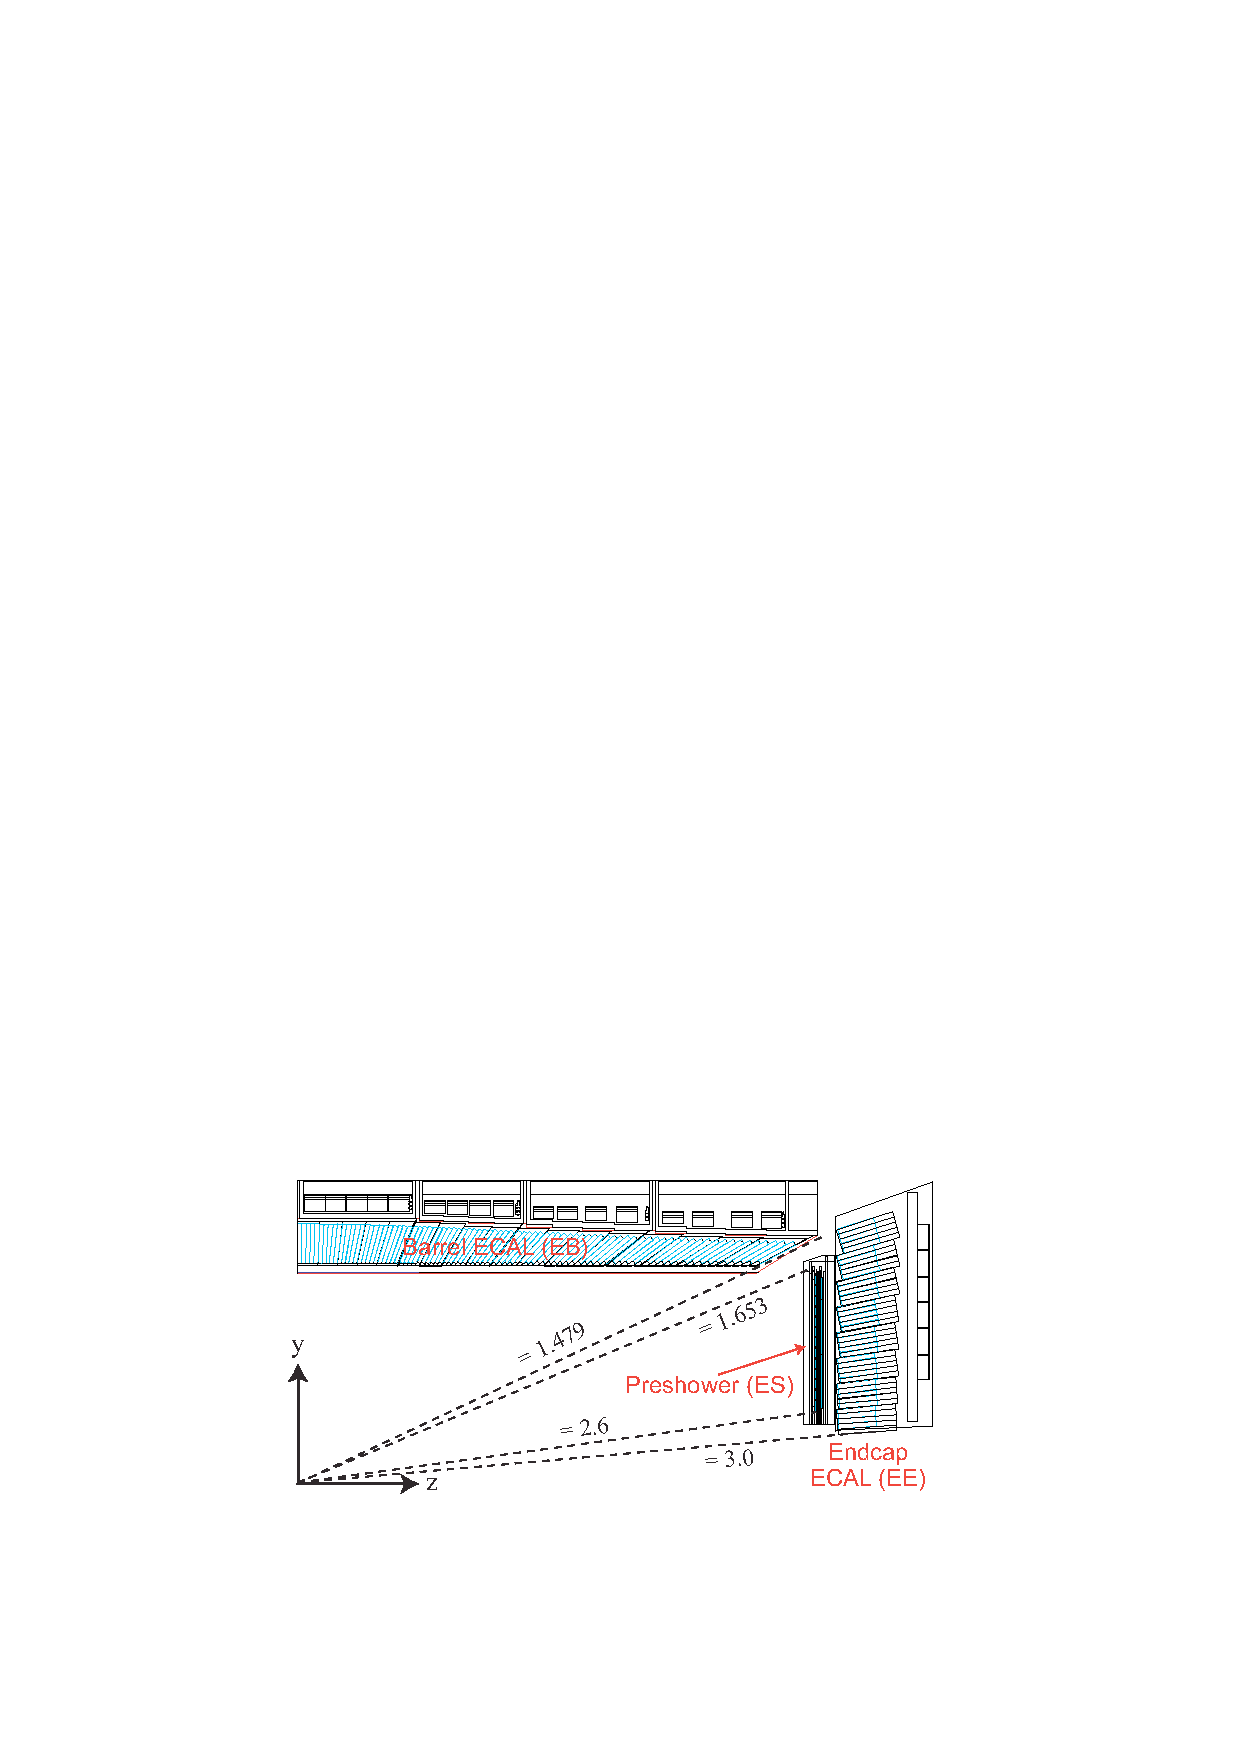
\includegraphics[scale = 1.2]{/home/anter/Desktop/Thesis/Figures/cropped_ECAL.pdf}\\
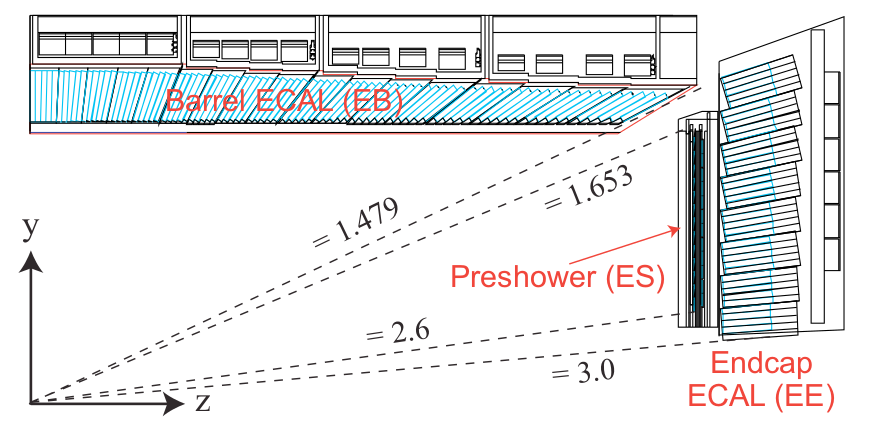
\includegraphics[scale = 0.6]{/home/anter/Desktop/Thesis/Figures/Final/ECAL.png}\\
\vspace*{0mm}
\caption[A geometric view of one quarter of the electromagnetic calorimeter (ECAL) in $y$-$z$ plane.]{A geometric view of one quarter of the electromagnetic calorimeter (ECAL) in $y$-$z$ plane showing the arrangement of sub-modules covering the barrel region (EB) and the endcaps (EE). ECAL is complemented with preshower detector (ES) mounted in front of the endcaps. Taken from \cite{Bayatian:2006nff}.}
\label{fig:ecal}
\end{center}
\end{figure}

The relative energy resolution of the ECAL has been measured to be \cite{Adzic:2007mi} :
\begin{equation}
{\rm \bigg(\frac{\sigma(E)}{E}\bigg)^2 = \bigg(\frac{2.8\%}{\sqrt{E}}\bigg)^2 \plus \bigg(\frac{12\%}{E}\bigg)^2 \plus \bigg(0.30\%\bigg)^2}
\end{equation}
where E is the energy in GeV. The first term is the stochastic component caused by fluctuations in the energy deposited in the preshower absorber and lateral shower containment. The second term is the contribution by noise and the last is the constant term which comes from leakage of energy from the back of the crystal, inter-calibration errors and non-uniformity of the longitudinal light collection. 

\subsection{Hadronic Calorimeter}
At CMS, the major fraction of the particles produced in proton-proton collisions is hadrons. These are usually collimated in a given direction producing conical structures called jets. The jets have both hadronic (charged and neutral) and electromagnetic components which are detected and measured by the combined CMS calorimeter system. The calorimeters are designed in a way that a particle loses all of its energy as it travels through them. The calorimeters measure the energies and directions of particle jets which indirectly give the energies and directions of quarks, gluons and neutrinos, initiating the jets. The energy deposits and the locations of these deposits are used to determine the directions and momenta of charged particles. But the neutral hadrons do not leave any track and hence their energy cannot be measured directly. The energy of neutral hadrons is measured by taking into account the missing transverse energy (\ETmiss). The determination of \ETmiss is a crucial tool in searching the new particles and new physics phenomena. Here, the hadron calorimeter (HCAL) comes into play which can detect neutral particles with non-zero mass such as neutrons. Since the neutral hadrons carry $\sim$10\% energy of the total jet energy, HCAL is an essential sub-system of the CMS detector and contributes to most of CMS's physics studies.

HCAL is a sampling calorimeter installed inside the solenoid coil. It consists of a non-magnetic brass absorber with a short interaction length of $\lambda_I$ = 16 cm and is interleaved with plastic scintillators having wavelength-shifting (WLS) fibres as readout. The highly energetic hadrons further produces a large number of pions and nucleons by inelastic interactions. The hadronic shower spreads more than the electromagnetic showers because of large transverse momentum of the secondary particles. As the energy of the particles is lower than a certain threshold, the ionization and low-energy hadronic processes come into play. The active scintillation material excites and blue-violet light is emitted. 
\begin{figure}[!h]
\begin{center}
\vspace*{3mm} 
\hspace*{-5mm}
%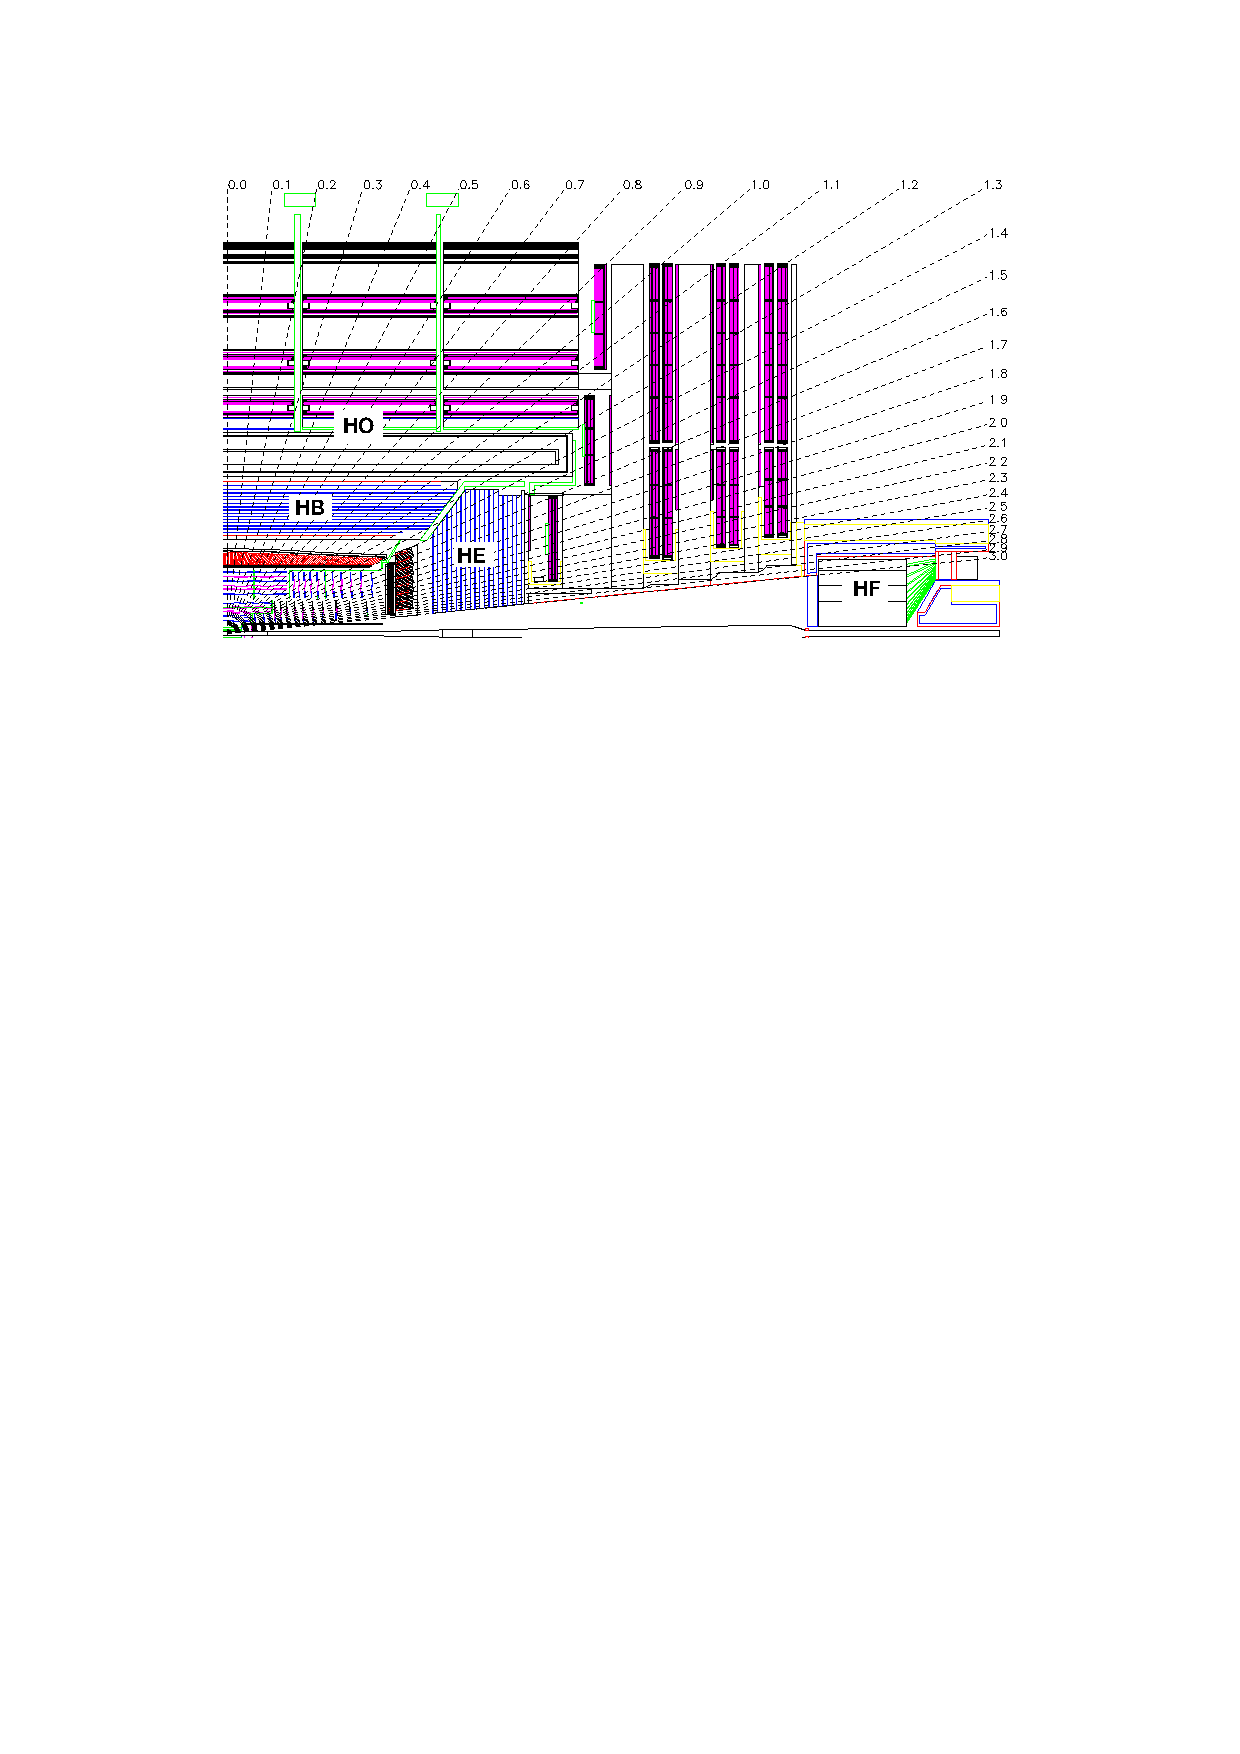
\includegraphics[scale = 1.]{/home/anter/Desktop/Thesis/Figures/edited_cropped_HCAL.pdf}\\
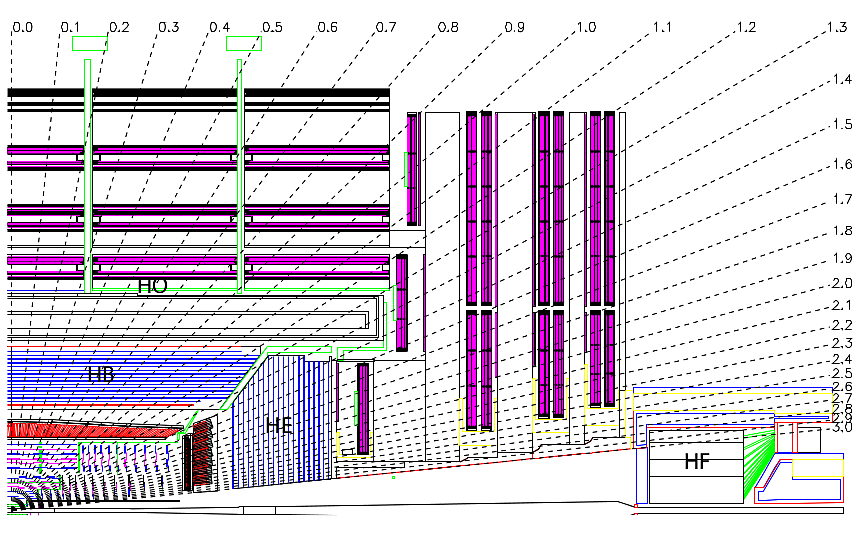
\includegraphics[scale = 0.6]{/home/anter/Desktop/Thesis/Figures/Final/HCAL.png}\\
\vspace*{4mm}
\caption[Longitudinal section of one quarter of the hadronic calorimeter (HCAL) in $r$-$\eta$ plane.]{Longitudinal section of one quarter of the hadronic calorimeter (HCAL) in $r$-$\eta$ plane. It consists of different parts : hadron barrel (HB), hadron outer (HO), hadron endcap (HE) and hadron forward (HF). Taken from \cite{Chatrchyan:2008aa}.}
\label{fig:hcal}
\end{center}
\end{figure}
The wavelength shifters connect all scintillators to photodiodes and read out the signals and further pass them to the data acquisition system. The longitudinal view of one quarter of the HCAL presented in Fig.~\ref{fig:hcal} shows the different parts : \\\newline
{\bf Hadron Barrel -} The hadron barrel (HB) is divided into two identical half barrel sections on either side of the interaction point. Each half barrel is made of 18 azimuthal wedges which are further divided into four azimuthal sectors each giving a granularity of $\Delta\phi$ = 0.087. In $z$ direction, the plastic scintillators are divided into 16 intervals of granularity $\Delta\eta$ = 0.087. HB covers the region up to $|\eta|$ \ls 1.305 and overlaps with endcaps for 1.305 $\leq~|\eta|~\leq$ 1.392. Since HB has the highest resolution $(\Delta\eta~\times~\Delta\phi = 0.087~\times~0.087$), it is optimal for calibration of the jet energy scale. The thickness of the HCAL amounts to 7-11 interaction lengths which are sufficient enough to absorb most of the hadrons.\\\newline
{\bf Hadron Outer -} The total amount of material in barrel region to absorb the hadronic shower is not sufficient. This requirement is fulfilled by placing an outer hadron (HO) calorimeter as a tail catcher on top of the coil of the magnet. The HO uses the solenoid coil as an additional absorber having interaction lengths of 1.4/sin$\theta$ and measures the tails of hadron showers penetrating the HB and the coil. Since the HO is physically located inside the muon system, it is strongly constrained by its geometry. The muon system is subdivided into 5 rings along the $z$-axis. Each of these rings is 2.536 m wide in $z$-direction and the HO is placed as first sensitive layer in these rings, with a scintillator thickness of 10 mm. The central ring ($\eta$ = 0) has two scintillator layers placed on each side of 19.5 cm thick iron layer.\\ \newline
{\bf Hadron Endcap -} The hadron endcaps (HE) extend the pseudorapidity range up to $|\eta|$ \ls 3.0. About 34\% of the particles produced in the final state reach this region. The granularity in $\Delta\eta~\times~\Delta\phi$ is 0.087 $\times$ 0.087 up to $|\eta|$ \ls 1.6 and 0.17 $\times$ 0.17 for $|\eta|$ \gr 1.6. The main challenges faced in the construction of the HE were the use of non-magnetic material in order to not disturb the magnetic field and the close distance to the beam line. The continuous damages caused by radiations decrease the detector response which should be monitored at regular intervals. \\ \newline
{\bf Hadron Forward -} The hadron forward (HF) calorimeter lies at a distance of $z$ = $\pm$11.2 m from the interaction point, covering the 2.8 \ls $|\eta|$ \ls 5.2 region. The HF has a cylindrical structure with an outer radius of 130.0 cm. It is azimuthally subdivided into 36, 20$\degree$ modular wedges. The HF is made up of 5 mm thick grooved steel plates which have quartz fibers inserted into the grooves. The fibres running parallel to the beam line are bundled to form 0.175 $\times$ 0.175 ($\Delta\eta~\times~\Delta\phi$) towers. The HF detects the jets having very high $\eta$ and also the hadronization products of the beam remnants. The iron absorbers and quartz fibers act as active material to measure the emitted Cerenkov light and to produce the signal in the photomultipliers (PMT).

%HCAL provides the energy and direction measurements of the jets in conjunction with ECAL system. It measures the total visible and missing transverse energy due to hermetic coverage.
The relative hadronic energy resolution of the barrel HCAL and ECAL combination can be parametrized as :
\begin{equation}
{\rm \bigg(\frac{\sigma(E)}{E}\bigg)^2} = \bigg(\frac{a}{\sqrt{\rm E}}\bigg)^2 \plus b^2
\end{equation}
where $a$ is a stochastic term and $b$ is a constant term. These values have been measured \cite{Chatrchyan:2009ag} as $a$ = (0.847$\pm$0.016) $\sqrt{\rm GeV}$ and $b$ = 0.074 $\pm$ 0.008 whereas for HF the measured values are $a$ = 1.98 $\sqrt{\rm GeV}$ and $b$ = 0.09.

\subsection{Superconducting Magnet}
The superconducting magnet is an essential feature of the CMS detector which is 13m long and 6m in diameter. Its refrigerated superconducting high-purity aluminium-stabilized niobium-titanium coils cooled at 4 Kelvin produces a magnetic field of 4 Teslas (T). The magnet will run at 3.8 T in order to maximize its lifetime. This intense solenoidal field makes the compactness and cylindrical symmetry of the detector possible. The magnet is placed between the calorimeters and the muon system. The solenoidal magnetic field parallel to the beam bends the tracks of the high momentum charged particles in the transverse plane. The curvature of the trajectory increases with the strength of the magnetic field which make possible to determine the transverse momentum more precisely. The magnet is complemented by an iron yoke ($\sim$10000 tonnes) which returns the magnetic field at 2 T.

\subsection{Muon System}
As the name of CMS suggests, the detection of muons is of central importance in the CMS detector. Out of all the known stable particles, only the muons and neutrinos pass through the calorimeter without depositing their energies. They interact very little with matter and can travel long distances through the dense matter. The charged muons can be detected by having an additional tracking system outside the calorimeters whereas the neutrinos are practically undetectable as they escape completely without being tracked in any of the layers of the calorimeters. Their presence can be detected from the missing energy carried by them. The CMS muon system is installed outside the calorimeters in the iron return yoke of the magnet which acts as a hadron absorber for the identification of the muons. Along with the muon identification, the muon system also measures their momenta and is also used for the triggering purposes. Good muon momentum resolution and trigger capability are enabled by the high-field solenoidal magnet and its flux-return yoke. The CMS muon system measures the momenta and charge of muons over the entire kinematic range of the LHC. The muon system shown in Fig.~\ref{fig:muon} consists of three types of gaseous particle detectors : \\ \newline
\begin{figure}[!t]
\begin{center}
\vspace*{3mm} 
\hspace*{-5mm}
%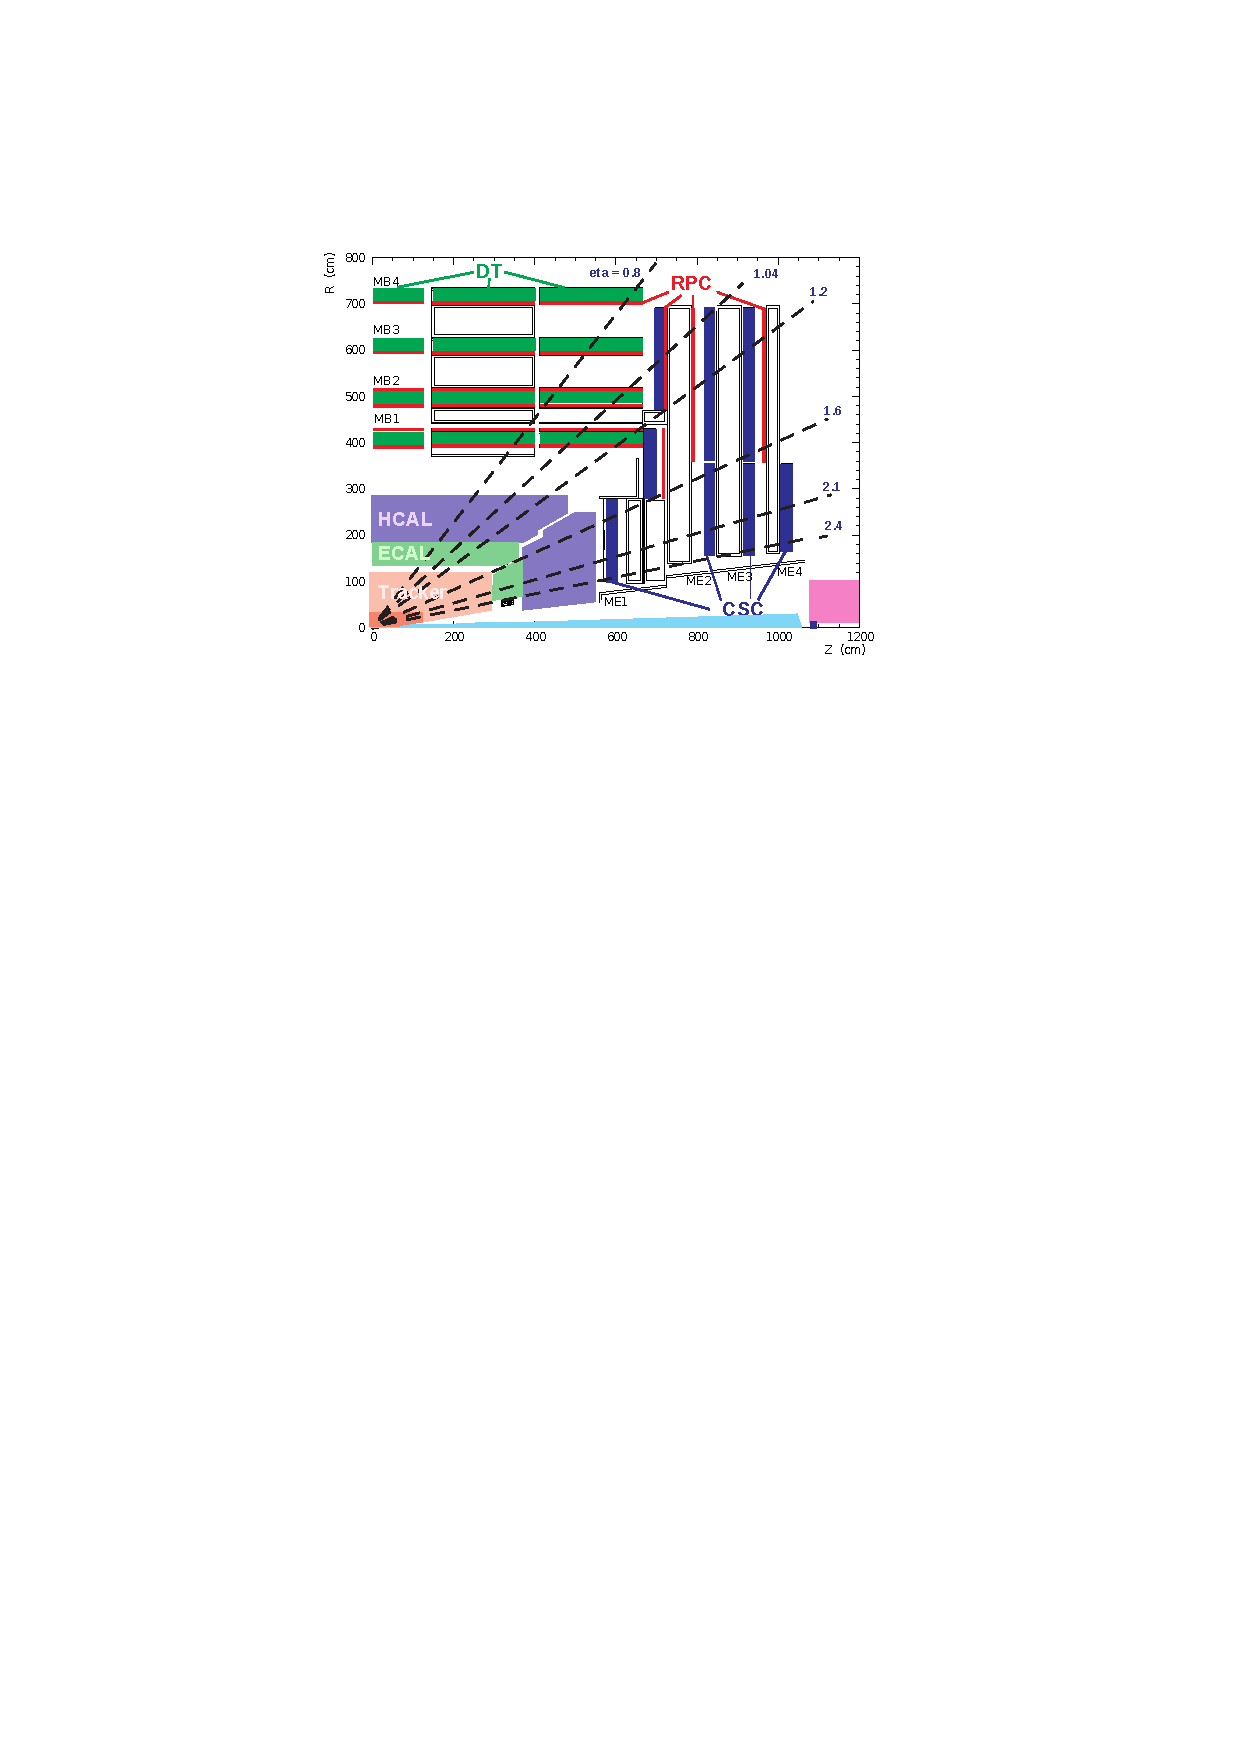
\includegraphics[scale = 1.4]{/home/anter/Desktop/Thesis/Figures/cropped_Muon.pdf}\\
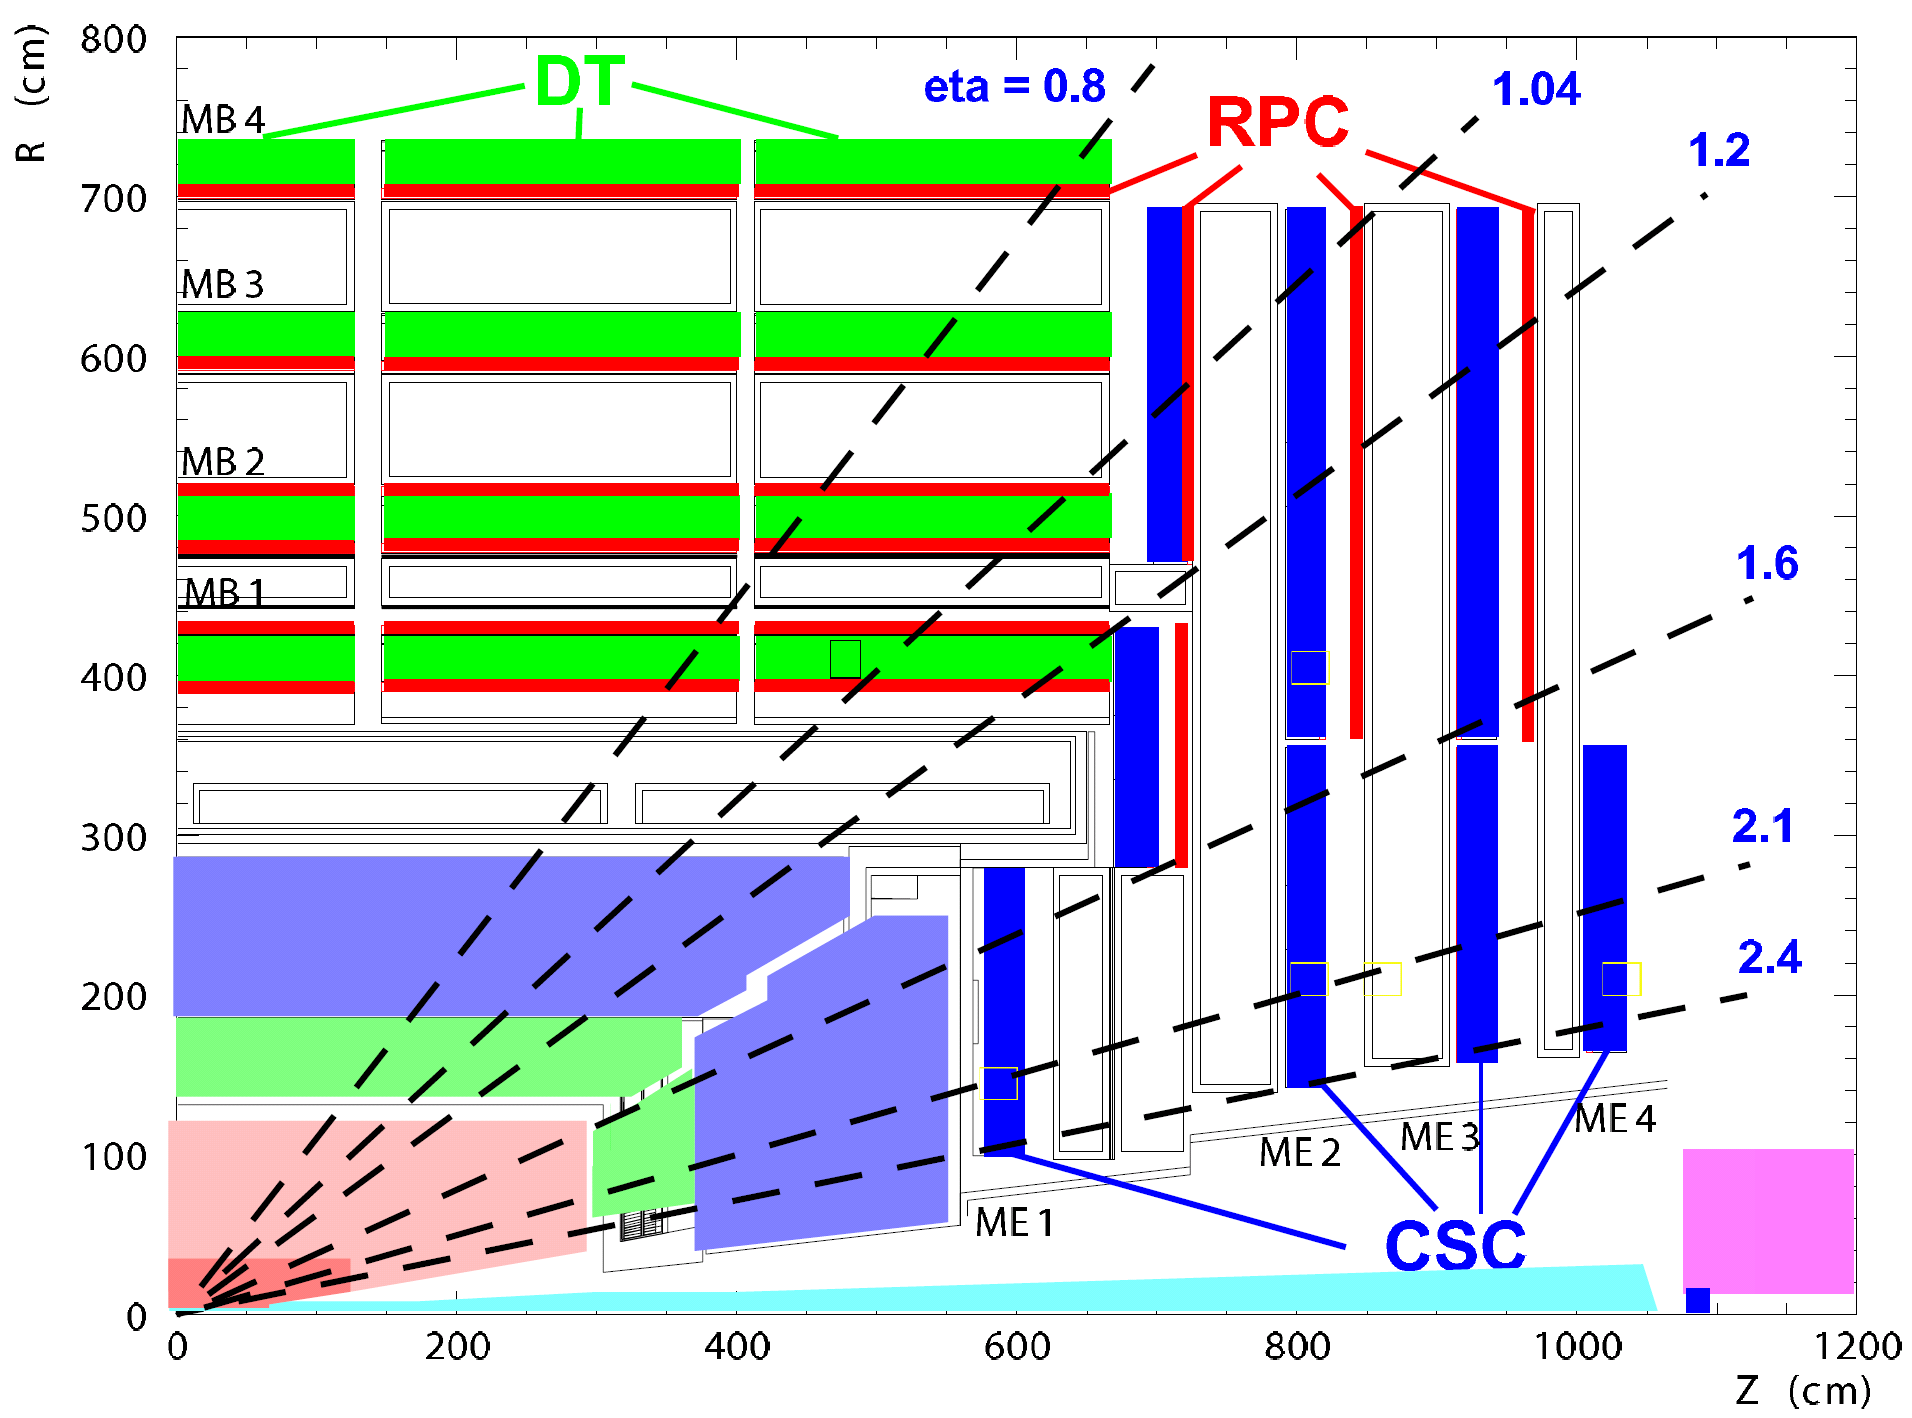
\includegraphics[scale = 0.83]{/home/anter/Desktop/Thesis/Figures/Final/Muon.png}\\
\vspace*{4mm}
\caption[A longitudinal view of the CMS muon system showing the location of the three gaseous particle detectors.]{A longitudinal view of the CMS muon system showing the location of the three gaseous particle detectors : four Drift Tube (DT) stations in the barrel (MB1-MB4, green), four stations of Cathode Strip Chambers (CSC) in the endcap (ME1-ME4, blue), and the Resistive Plate Chambers (RPC) stations (red)\footnotemark.}
\label{fig:muon}
\end{center}
\end{figure}
{\bf Drift Tube -} 
The muon barrel (MB) detector has four concentric layers of drift tube (DT) chambers inside the iron yoke which covers the region up to $|\eta|$ \ls 1.2. DT stations are distributed into 5 wheels along the $z$ direction. Each wheel is divided into 12 sectors, each sector covering a 30$\degree$ azimuthal angle. The DT is an aluminium tube having length of 2.5 m and area of 4.2 $\times$ 1.3 cm$^{2}$. It is filled with a gas mixture consisting of 58\% Ar \plus 15 \% CO$_{2}$. \\ \newline
{\bf Cathode Strip Chambers -} In the forward region, the muon and background flux is higher. In this region, cathode strip chambers (CSC) are preferred because of their fast response time, high radiation tolerance and fine segmentation. In each end cap, four stations of CSCs are installed which cover the region of 0.9 \ls $|\eta|$ \ls 2.4. Each CSC is trapezoidal in shape and consists of 6 gas gaps. Each gap has a plane of radial cathode strips and a plane of anode wires lying in perpendicular direction to the strips. \\ \newline 
{\bf Resistive Plate Chambers -} Both DT and CSC are accompanied by resistive plate chambers (RPC) which are double-gap chambers. RPCs operate in avalanche mode to ensure good performance at high rates. They help to resolve ambiguities in attempting to make tracks from multiple hits in a chamber. They also provide additional points for determination of a muon trajectory and give fast response to the trigger system which is described in the following section.
\footnotetext{Source : \url{https://arxiv.org/abs/1209.2646}}
\subsection{Trigger and Data Acquisition System}
At the LHC, the interaction rates in proton-proton collisions are very high. In the 2012 run period, the beam crossing frequency was 25 ns. At this frequency, around 40 million bunch crossings occur per second with an average of around 20 collisions per bunch crossing. But the rate at which the information can be stored is much lower than collision rates. Hence, either the storage rate should be increased or event rates should be decreased. This is achieved by using an efficient trigger system which retains the interesting signal events and rejects the background events. An event should be accepted or rejected very quickly, based on signals of certain physics objects inside the detector.
CMS has a two-level complex trigger system : \\\newline
{\bf Level-1 Trigger -} The Level-1 (L1) trigger system is based on custom electronics which stores the events at maximum rate of 100 kHz and then forward them to the next level triggers. The L1 system uses only coarsely segmented data from calorimeter and muon detectors and holds all the high-resolution data in pipeline memories in the front-end electronics. The work flow of the L1 trigger system, consisting of local, regional and global components, is shown in Fig.~\ref{fig:L1}.
\begin{figure}[!h]
\begin{center}
\vspace*{3mm} 
\hspace*{-5mm}
%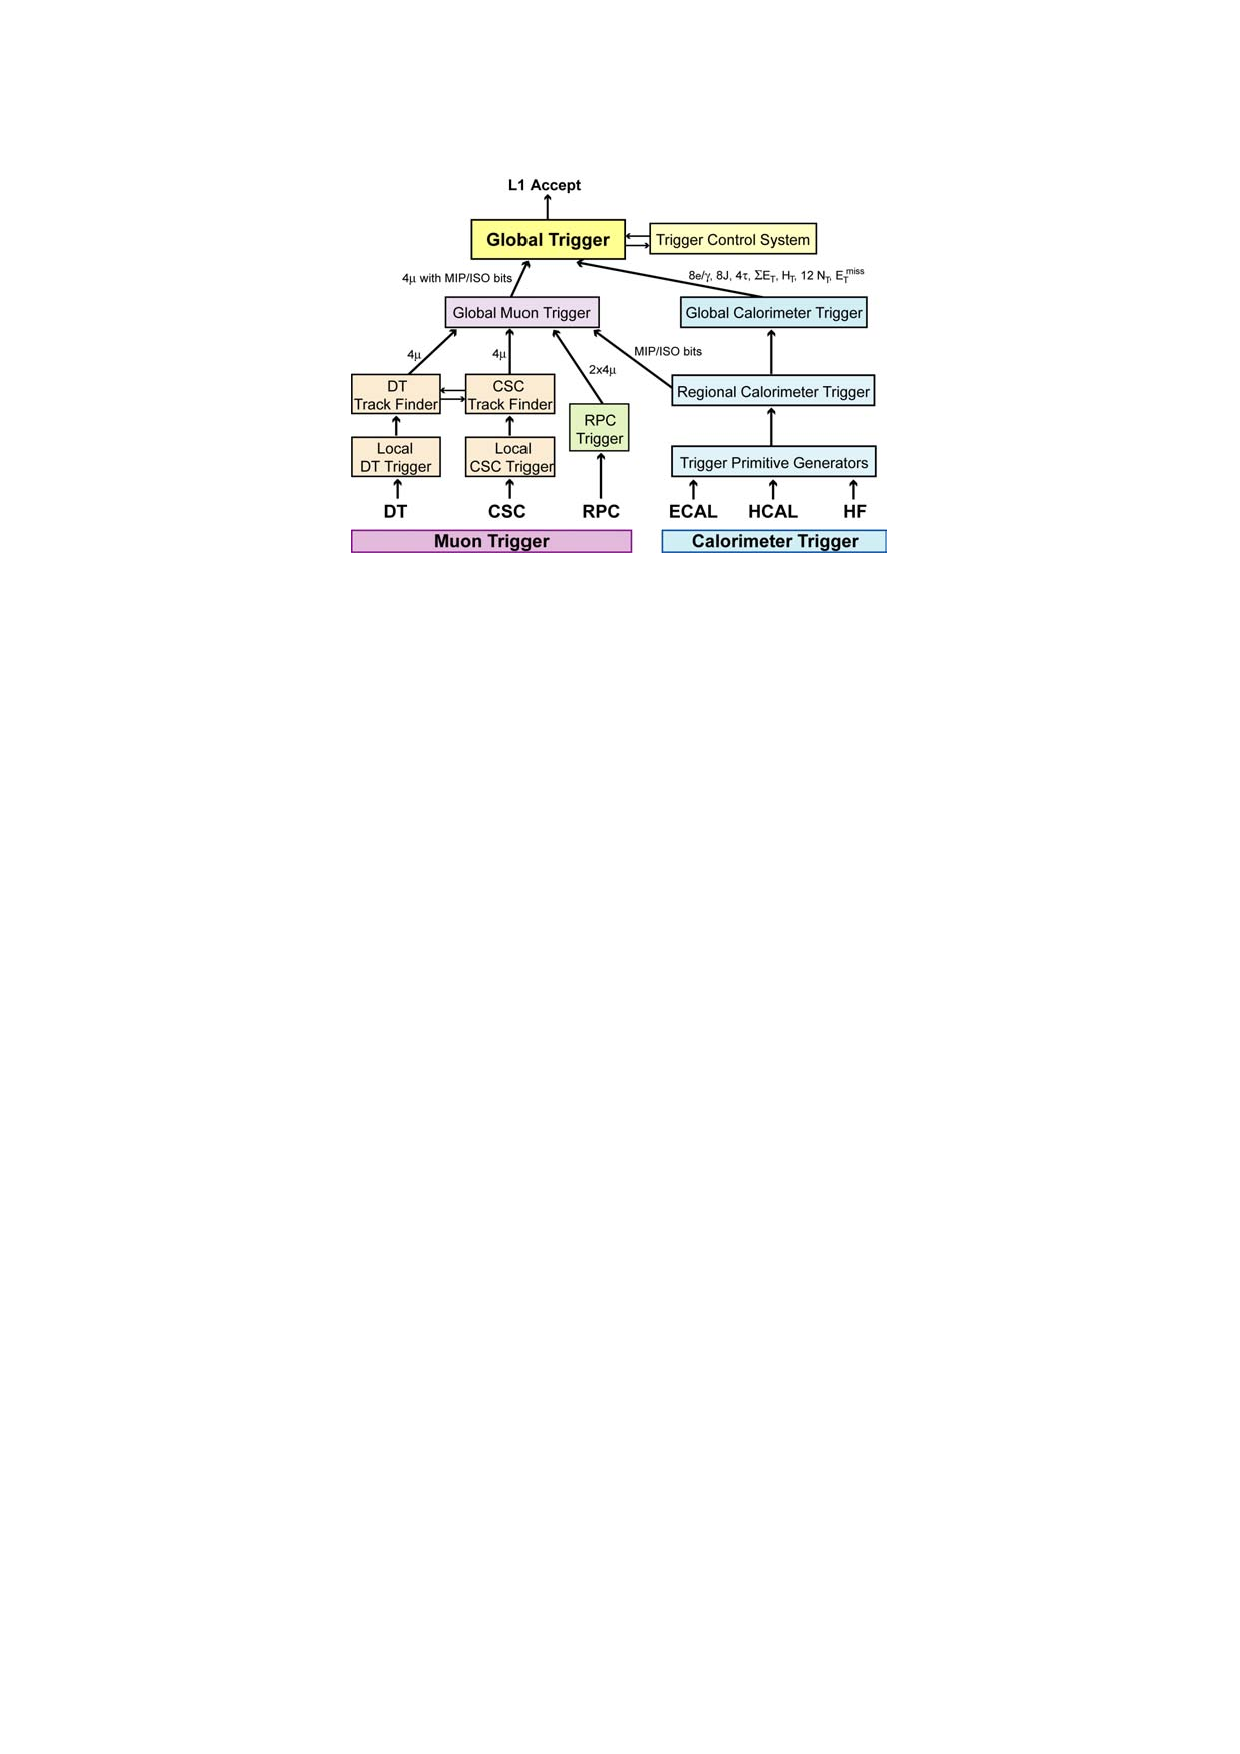
\includegraphics[scale = 1.5]{/home/anter/Desktop/Thesis/Figures/cropped_Trigger.pdf}\\
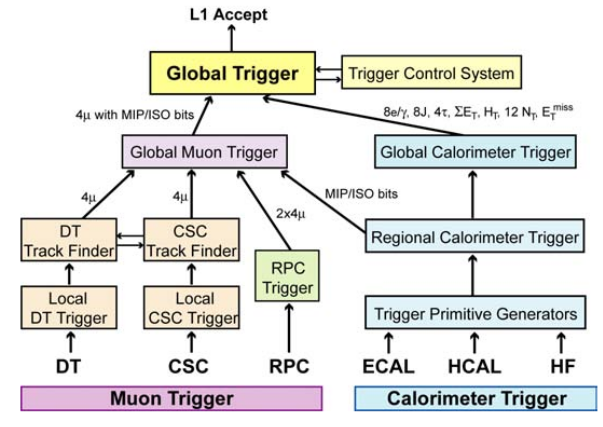
\includegraphics[scale = 0.85]{/home/anter/Desktop/Thesis/Figures/Final/Trigger.png}\\
\vspace*{4mm}
\caption[Work flow of the L1 trigger system consisting of local, regional and global components.]{Work flow of the L1 trigger system consisting of local, regional and global components. Taken from \cite{Chatrchyan:2008aa}.}
\label{fig:L1}
\end{center}
\end{figure}
The local triggers known as Trigger Primitive Generators are based on energy deposits in calorimeter trigger towers and tracks in muon chambers. The Regional Triggers combine their information and use pattern logic to determine ranked and sorted trigger objects such as electron or muon candidates in limited spatial regions. The rank is determined as a function of energy or momentum and quality, which reflects the level of confidence attributed to the L1 parameter measurements, based on detailed knowledge of the detectors and trigger electronics and on the amount of information available. The Global Calorimeter and Global Muon Triggers determine the highest-rank calorimeter and muon objects and transfer them to the Global Trigger (GT), the top entity of the Level-1 hierarchy. The events accepted by the GT are further evaluated by the HLT. \\\newline
{\bf High Level Trigger -} At the second step, a software-based High-Level Trigger (HLT) reduces the maximum L1 accepted rate of 100 kHz to a final output rate of 100 Hz. The HLT system filters events by performing physics selections based on the offline reconstruction software. The on-line processor farm provides the HLT and a fraction of the accepted events are passed to the Data Acquisition (DAQ) system for further processing.

\subsubsection{Jet Triggers}
\begin{comment}
\begin{figure}[!h]
\begin{center}
\vspace*{3mm} 
\hspace*{-5mm}
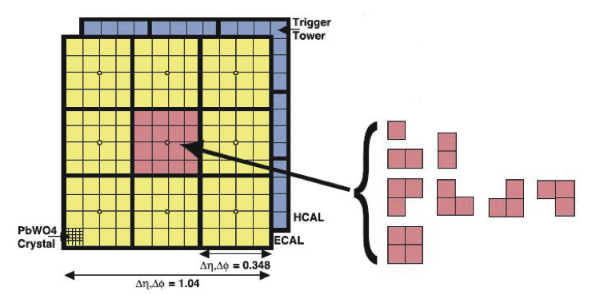
\includegraphics[scale = 0.7]{/home/anter/Desktop/Thesis/Figures/Jet_trigger.png}\\
\vspace*{4mm}
\caption[Muon]{Illustration of the available tower granularity for the L1 jet finding algorithm in the
central region, |η|<3 (left). The jet trigger uses a 3×3 calorimeter region sliding window technique which spans the full(η,φ)coverage of the calorimeter. The active tower patterns allowed for L1τjet candidates are shown on the right Work flow of the L1 trigger system \cite{Chatrchyan:2008aa}.}
\label{fig:Jettrigger}
\end{center}
\end{figure}
\end{comment}
At CMS, there are various types of triggers depending on the analysis to be performed. The triggers based on jet properties and missing transverse energy (\ETmiss) are important for search for new physics whereas the single-jet triggers are mainly designed to study quantum chromodynamics (QCD). This thesis uses the single-jet triggers to select the events for analysis. At L1, the single-jet triggers use information mainly from the calorimeters by looking for the highest energy deposit. The sums of transverse energy from ECAL and HCAL are computed in 4 $\times$ 4 trigger towers, except in the HF region where this quantity is measured in the whole trigger tower itself. If the calculated sum is greater than a certain threshold, the event is selected at L1 and it is passed to the HLT. At HLT level, the jets are reconstructed using the anti-\kt jet clustering algorithm. The inputs to the jet algorithm are either calorimeter towers giving ``CaloJet'' objects, or the reconstructed particle flow objects giving ``PFJet'' objects. The processing of reconstruction algorithm takes a long time and hence the jet trigger paths are divided into multiple selection steps. At first, the jets are reconstructed from calorimeter towers. The PF algorithm is run only for events in which at least one calorimeter jet passes a certain \pt threshold. The jets are then again clustered again from the PF candidates. In 2012, most of the jet trigger paths take PFJets as their inputs. The rate of jet events is quite high, so PFJet trigger paths have a pre-selection based on CaloJets. The matching between CaloJets and PFJets is required in single PFJet paths. Due to the flexibility of the HLT, it is possible to apply the jet energy corrections during the HLT selection.

\subsubsection{Data Acquisition System}
As the L1 trigger accepts events at a rate of 100 kHz, the Data Acquisition (DAQ) system has to process the events at the same speed. It reads out the data of all detector sub-components and assembles the complete events, see Fig.~\ref{fig:DAQ}. The data is subsequently passed to the HLT which further reduces the rates to a few hundred events per second. Finally, the events are merged and saved to a local storage system, from which they are continuously transferred to the Tier-0 computing center at CERN.

\begin{figure}[!h]
\begin{center}
\vspace*{1mm} 
\hspace*{-5mm}
%includegraphics[scale = 1.3]{/home/anter/Desktop/Thesis/Figures/cropped_DAQ.pdf}\\
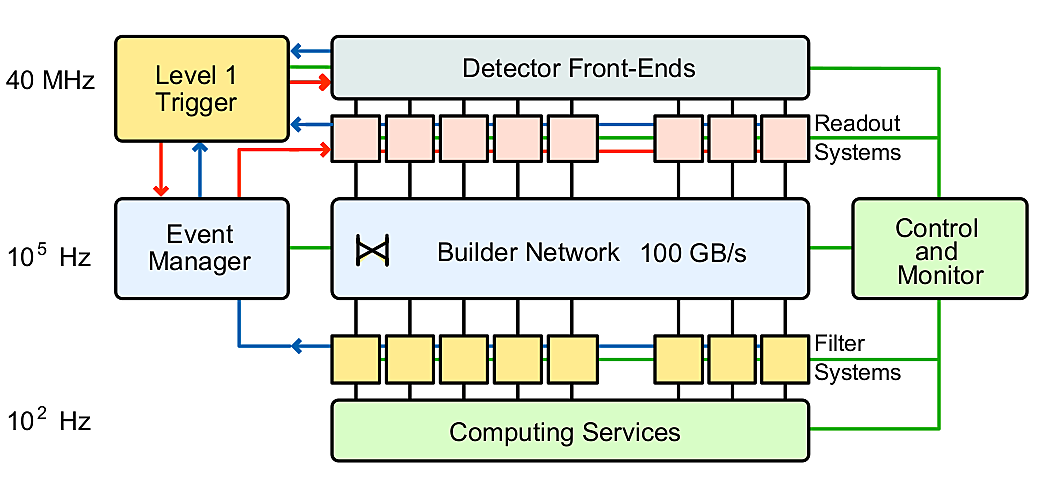
\includegraphics[scale = 0.5]{/home/anter/Desktop/Thesis/Figures/Final/DAQ.png}\\
\vspace*{2mm}
\caption[Architecture of the CMS Data Acquisition (DAQ) system.]{Architecture of the CMS Data Acquisition (DAQ) system. Taken from \cite{Chatrchyan:2008aa}.}
\label{fig:DAQ}
\end{center}
\end{figure}

\subsection{Data Management}
Although the trigger system reduces the collision rate enough to be stored, still there is a huge amount of the data need to be analyzed. An efficient computing infrastructure and the software is required for storing and distributing the data. To meet this need, the LHC has a data storage infrastructure called the Worldwide LHC Computing Grid (WLCG) \cite{Bird:2005js}. WLCG provides a hierarchical structure, as shown in Fig.~\ref{fig:Computing}, in a series of four levels or Tiers. Each Tier is made up of several computer centres. All the raw collision data collected by CMS is converted into a format suitable for offline analysis and sorted in the form of the data sets at the Tier-0 site at CERN. This processed data is then transferred to Tier-1 centers all over the world where reconstruction algorithms are run. Further reconstructed and simulated data is distributed to Tier-2 sites, where it is available for physics analysis mainly performed on Tier-3 sites. %The powerful Monte Carlo event generators are required to simulate the collision events and these are dicussed in the next chapter.

\begin{figure}[!h]
\begin{center}
\vspace*{3mm} 
\hspace*{-5mm}
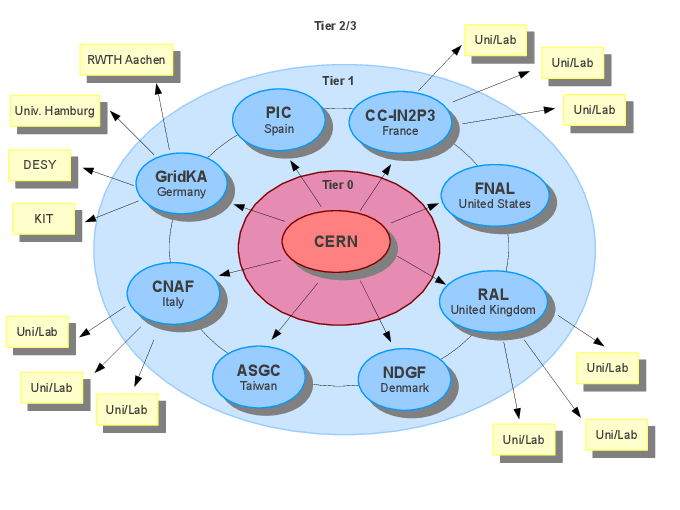
\includegraphics[scale = 0.95]{/home/anter/Desktop/Thesis/Figures/Computing.png}\\
\vspace*{4mm}
\caption[The schematic overview of the CMS computing grid.]{The schematic overview of the CMS computing grid. All data collected by CMS is stored at the Tier-0 site at CERN which is then transferred to Tier-1 centers all over the world. Further reconstructed and simulated data is distributed to Tier-2 sites, where it is available for physics analysis mainly performed on Tier-3 sites. Taken from \cite{Bird:2005js}.}
\label{fig:Computing}
\end{center}
\end{figure}

\section{Software Tools}
Every year, the CMS is recording a huge amount of collision and simulation data. This data is analyzed iteratively to improve the understanding of the detector and the measured physics. So a dedicated data structure and software tools are required for data analysis. These are included in the software framework referred to as CMSSW framework.

%CMSSW has also some pre-defined data tier, i.e sets with specific objects. Among them are the data tier RECO which included all reconstructed data objects, whereas the data tier AOD (Analysis Object Data) is only a subset with physical objects needed for a particular analysis.
\subsection{CMSSW Framework}
The CMS software framework (CMSSW) \cite{CMS:2005aa} provides all necessary tools required to perform a physics analysis. It is built on top of an event data model (EDM). It is a container for arbitrary C\plusn\plus objects, e.g. recorded raw data and reconstructed physical objects or derived physical quantities of an event. The reconstruction algorithms in the CMSSW framework are divided into modules, which can be dynamically loaded and run. The event processing model in CMSSW is run by one executable, called cmsRun. SCRAM (Source Configuration, Release, And Management) is a configuration and management tool in the framework. It builds a runtime environment and make available all the necessary shared libraries. The shared libraries reduces memory consumption by loading only required modules during runtime. The CMSSW framework performs calibration, event generation, detector simulation, event reconstruction as well as data analysis by implementing the codes either in C\plusn\plus or Python languages. To reduce the event content, a process called skimming is performed where only necessary data is preserved. 

\subsection{ROOT}
ROOT \cite{Brun:1997pa} is an open source object-oriented data analysis framework, developed by CERN. It consists of a huge C\plusn\plus library provided with all the functionalities to store and analyze large amounts of the data. It provides histrogramming methods in 1, 2 and 3 dimensions, curve fitting functions, minimization procedures, graphics and visualization classes. The command language of ROOT is command line interpreter (CINT), with several extensions to C\plusn\plus which makes ROOT a versatile package. ROOT can be extended dynamically by linking external libraries. The events generated or analyzed in CMSSW framework are stored in a tree structure in files using ROOT libraries. In this thesis, ROOT has been used extensively for storing information of events or objects, for analyzing the events, for fitting as well as plotting purposes.

\subsection{\NLOJET~and \fastNLO}
\label{Sec:NLO}
The cross-sections for jet production at leading order (LO) and next-to-leading order (NLO) are evaluated using a C\plusn\plus program called \NLOJETPP \cite{Nagy:2001fj,Nagy:2003tz}. It uses the dipole subtraction method for the separation of the divergences and can calculate up to three-jet observables at NLO precision. The perturbative QCD cross-sections are calculated using Monte Carlo integration methods which are very time consuming. It makes PDF fits or estimations of uncertainties difficult where the calculations of the cross-sections are need to be repeated. So the \NLOJETPP is interfaced to the \fastNLO project \cite{Kluge:2006xs,Britzger:2012bs} which performs fast re-evaluations of cross-sections. It stores the perturbative coefficients obtained with \NLOJETPP in a way that the strong coupling constant and the PDFs can be changed afterwards without a recalculation of the perturbative coefficients.

All the event generators and cross-section calculation tools take the PDFs as an input. They are either hard coded in the generators or accessed via a standardized interface with the LHAPDF library \cite{Whalley:2005nh,Buckley:2014ana}. LHAPDF provides a unified and easy way to use the PDF sets by storing them in the data files. It provides interpolation routines to read the PDFs and interpolate the PDFs at all scales. It also allows access to single PDF members without needing to load whole sets. LHAPDF is supported by many MC event generators and other physics programs.

